\documentclass[modern,linenumbers,trackchanges]{aastex7}
%\usepackage{sansmath}
%\sansmath


\usepackage{amsmath} 
\usepackage{color}
\definecolor{black}{rgb}{0,0,0}
\definecolor{blue}{rgb}{0.2,0.2,0.81}
\definecolor{orange}{rgb}{0.92,0.33,0.16}

\definecolor{gray}{rgb}{.5,0.5,0.5}
\newcommand{\todo}[1]{{\color{orange}  #1 \normalfont}}
\newcommand{\zkbt}[1]{{\color{black} #1}\normalfont}
		
\begin{document}
%\title{The Slope of the Cosmic Shoreline is Terrifically Uncertain}
%\title{The Cosmic Shoreline is 3D}
%\title{The Cosmic Shoreline in 3D}
%\title{The Cosmic Shoreline is 3D}
\title{The 3D Cosmic Shoreline for Nurturing Planetary Atmospheres}
%sustaining? preserving? 

\shorttitle{Probabilistic Cosmic Shorelines}


\author[orcid=0000-0002-3321-4924,sname='Berta-Thompson']{Zach K. Berta-Thompson}
\affiliation{University of Colorado Boulder, Department of Astrophysical and Planetary Sciences}
\email[show]{zach.bertathompson@colorado.edu}  


\author[orcid=0000-0001-6484-7559,sname='Wachiraphan']{Patcharapol Wachiraphan}
\affiliation{University of Colorado Boulder, Department of Astrophysical and Planetary Sciences}
\email{patcharapol.wachiraphan@colorado.edu}  



\author[orcid=0000-0001-8504-5862,sname='Murray']{Catriona Murray}
\affiliation{University of Colorado Boulder, Department of Astrophysical and Planetary Sciences}
\email{catriona.murray@colorado.edu}  


% include variables that can be updated easily!
% mass-radius
\newcommand{\mrb}{-0.001 \pm 0.029}
\newcommand{\mrbjustvalue}{-0.001}
\newcommand{\mrbsigma}{-1.34 \pm 0.1}
\newcommand{\mrbsigmajustvalue}{-1.34}
\newcommand{\mrm}{3.4 \pm 0.032}
\newcommand{\mrmjustvalue}{3.4}
\newcommand{\mrmsigma}{-0.261 \pm 0.04}
\newcommand{\mrmsigmajustvalue}{-0.261}
\newcommand{\mrscatteratearth}{26.1 \pm 2.7}
\newcommand{\mrscatteratearthjustvalue}{26.1}
\newcommand{\mrscatteratsmall}{159_{-31}^{+41}}
\newcommand{\mrscatteratsmalljustvalue}{159}
\newcommand{\mrpowerRvesc}{0.835 \pm 0.011}
\newcommand{\mrpowerRvescjustvalue}{0.835}
\newcommand{\mrpowerMvesc}{2.83 \pm 0.011}
\newcommand{\mrpowerMvescjustvalue}{2.83}
\newcommand{\mrpowerp}{3.17 \pm 0.011}
\newcommand{\mrpowerpjustvalue}{3.17}

%all-any-uncertainties=True
\newcommand{\allanyTruelnw}{-1.26 \pm 0.32}
\newcommand{\allanyTruelnwjustvalue}{-1.26}
\newcommand{\allanyTruelogfo}{2.78_{-0.35}^{+0.52}}
\newcommand{\allanyTruelogfojustvalue}{2.78}
\newcommand{\allanyTruep}{6.08_{-0.48}^{+0.69}}
\newcommand{\allanyTruepjustvalue}{6.08}
\newcommand{\allanyTrueq}{1.25_{-0.22}^{+0.31}}
\newcommand{\allanyTrueqjustvalue}{1.25}
\newcommand{\allanyTruew}{0.284_{-0.075}^{+0.11}}
\newcommand{\allanyTruewjustvalue}{0.284}
\newcommand{\allanyTruefo}{598_{-3.3e+02}^{+1.4e+03}}
\newcommand{\allanyTruefojustvalue}{598}
\newcommand{\allanyTruelogLnohz}{-2.22 \pm 0.21}
\newcommand{\allanyTruelogLnohzjustvalue}{-2.22}
\newcommand{\allanyTrueLnohz}{0.006_{-0.002}^{+0.003}}
\newcommand{\allanyTrueLnohzjustvalue}{0.006}
\newcommand{\allanyTruewninetyfive}{1.67_{-0.44}^{+0.65}}
\newcommand{\allanyTruewninetyfivejustvalue}{1.67}
\newcommand{\allanyTruewninetyfiveasfluxfactor}{47_{-30}^{+1.6e+02}}
\newcommand{\allanyTruewninetyfiveasfluxfactorjustvalue}{47}
\newcommand{\allanyTrueqfromard}{1.63_{-0.2}^{+0.3}}
\newcommand{\allanyTrueqfromardjustvalue}{1.63}

%all-CO2-uncertainties=False
\newcommand{\allCOOFalselnw}{-1.82 \pm 0.47}
\newcommand{\allCOOFalselnwjustvalue}{-1.82}
\newcommand{\allCOOFalselogfo}{2.79_{-0.4}^{+0.58}}
\newcommand{\allCOOFalselogfojustvalue}{2.79}
\newcommand{\allCOOFalsep}{6.34_{-1.5}^{+2.1}}
\newcommand{\allCOOFalsepjustvalue}{6.34}
\newcommand{\allCOOFalseq}{1.32_{-0.3}^{+0.43}}
\newcommand{\allCOOFalseqjustvalue}{1.32}
\newcommand{\allCOOFalsew}{0.162_{-0.06}^{+0.1}}
\newcommand{\allCOOFalsewjustvalue}{0.162}
\newcommand{\allCOOFalsefo}{612_{-3.7e+02}^{+1.7e+03}}
\newcommand{\allCOOFalsefojustvalue}{612}
\newcommand{\allCOOFalselogLnohz}{-2.11 \pm 0.28}
\newcommand{\allCOOFalselogLnohzjustvalue}{-2.11}
\newcommand{\allCOOFalseLnohz}{0.008_{-0.004}^{+0.006}}
\newcommand{\allCOOFalseLnohzjustvalue}{0.008}
\newcommand{\allCOOFalsewninetyfive}{0.954_{-0.35}^{+0.59}}
\newcommand{\allCOOFalsewninetyfivejustvalue}{0.954}
\newcommand{\allCOOFalsewninetyfiveasfluxfactor}{8.98_{-5}^{+26}}
\newcommand{\allCOOFalsewninetyfiveasfluxfactorjustvalue}{8.98}
\newcommand{\allCOOFalseqfromard}{1.64_{-0.23}^{+0.34}}
\newcommand{\allCOOFalseqfromardjustvalue}{1.64}

%exo-any-uncertainties=True
\newcommand{\exoanyTruelnw}{-2.11_{-1.8}^{+0.65}}
\newcommand{\exoanyTruelnwjustvalue}{-2.11}
\newcommand{\exoanyTruelogfo}{3.13_{-0.57}^{+0.73}}
\newcommand{\exoanyTruelogfojustvalue}{3.13}
\newcommand{\exoanyTruep}{5.38_{-2.3}^{+3.1}}
\newcommand{\exoanyTruepjustvalue}{5.38}
\newcommand{\exoanyTrueq}{1.38_{-0.27}^{+0.43}}
\newcommand{\exoanyTrueqjustvalue}{1.38}
\newcommand{\exoanyTruew}{0.121 \pm 0.11}
\newcommand{\exoanyTruewjustvalue}{0.121}
\newcommand{\exoanyTruefo}{1.35e+03_{-9.9e+02}^{+6e+03}}
\newcommand{\exoanyTruefojustvalue}{1.35e+03}
\newcommand{\exoanyTruelogLnohz}{-2.27 \pm 0.36}
\newcommand{\exoanyTruelogLnohzjustvalue}{-2.27}
\newcommand{\exoanyTrueLnohz}{0.005_{-0.003}^{+0.007}}
\newcommand{\exoanyTrueLnohzjustvalue}{0.005}
\newcommand{\exoanyTruewninetyfive}{0.715 \pm 0.63}
\newcommand{\exoanyTruewninetyfivejustvalue}{0.715}
\newcommand{\exoanyTruewninetyfiveasfluxfactor}{5.18_{-3.9}^{+19}}
\newcommand{\exoanyTruewninetyfiveasfluxfactorjustvalue}{5.18}
\newcommand{\exoanyTrueqfromard}{1.84_{-0.33}^{+0.43}}
\newcommand{\exoanyTrueqfromardjustvalue}{1.84}

%solar-any-uncertainties=False
\newcommand{\solaranyFalselnw}{-1.37 \pm 0.66}
\newcommand{\solaranyFalselnwjustvalue}{-1.37}
\newcommand{\solaranyFalselogfo}{0.865_{-0.41}^{+0.56}}
\newcommand{\solaranyFalselogfojustvalue}{0.865}
\newcommand{\solaranyFalsep}{3.76_{-0.51}^{+0.73}}
\newcommand{\solaranyFalsepjustvalue}{3.76}
\newcommand{\solaranyFalseq}{0.003 \pm 0.93}
\newcommand{\solaranyFalseqjustvalue}{0.003}
\newcommand{\solaranyFalsew}{0.254_{-0.12}^{+0.25}}
\newcommand{\solaranyFalsewjustvalue}{0.254}
\newcommand{\solaranyFalsefo}{7.34_{-4.5}^{+19}}
\newcommand{\solaranyFalsefojustvalue}{7.34}
\newcommand{\solaranyFalselogLnohz}{-0.01 \pm 2.7}
\newcommand{\solaranyFalselogLnohzjustvalue}{-0.01}
\newcommand{\solaranyFalseLnohz}{0.977_{-0.97}^{+5.5e+02}}
\newcommand{\solaranyFalseLnohzjustvalue}{0.977}
\newcommand{\solaranyFalsewninetyfive}{1.5_{-0.69}^{+1.5}}
\newcommand{\solaranyFalsewninetyfivejustvalue}{1.5}
\newcommand{\solaranyFalsewninetyfiveasfluxfactor}{31.4_{-25}^{+9.3e+02}}
\newcommand{\solaranyFalsewninetyfiveasfluxfactorjustvalue}{31.4}
\newcommand{\solaranyFalseqfromard}{0.509_{-0.24}^{+0.33}}
\newcommand{\solaranyFalseqfromardjustvalue}{0.509}

%exo-any-uncertainties=False
\newcommand{\exoanyFalselnw}{-1.7 \pm 0.45}
\newcommand{\exoanyFalselnwjustvalue}{-1.7}
\newcommand{\exoanyFalselogfo}{3.17_{-0.54}^{+0.76}}
\newcommand{\exoanyFalselogfojustvalue}{3.17}
\newcommand{\exoanyFalsep}{5.03_{-2.1}^{+3}}
\newcommand{\exoanyFalsepjustvalue}{5.03}
\newcommand{\exoanyFalseq}{1.4_{-0.28}^{+0.43}}
\newcommand{\exoanyFalseqjustvalue}{1.4}
\newcommand{\exoanyFalsew}{0.182_{-0.066}^{+0.11}}
\newcommand{\exoanyFalsewjustvalue}{0.182}
\newcommand{\exoanyFalsefo}{1.48e+03_{-1.1e+03}^{+7e+03}}
\newcommand{\exoanyFalsefojustvalue}{1.48e+03}
\newcommand{\exoanyFalselogLnohz}{-2.29 \pm 0.36}
\newcommand{\exoanyFalselogLnohzjustvalue}{-2.29}
\newcommand{\exoanyFalseLnohz}{0.005_{-0.003}^{+0.007}}
\newcommand{\exoanyFalseLnohzjustvalue}{0.005}
\newcommand{\exoanyFalsewninetyfive}{1.07_{-0.39}^{+0.63}}
\newcommand{\exoanyFalsewninetyfivejustvalue}{1.07}
\newcommand{\exoanyFalsewninetyfiveasfluxfactor}{11.9_{-7}^{+38}}
\newcommand{\exoanyFalsewninetyfiveasfluxfactorjustvalue}{11.9}
\newcommand{\exoanyFalseqfromard}{1.86_{-0.32}^{+0.45}}
\newcommand{\exoanyFalseqfromardjustvalue}{1.86}

%solar-CO2-uncertainties=True
\newcommand{\solarCOOTruelnw}{-2.13_{-1.9}^{+2.7}}
\newcommand{\solarCOOTruelnwjustvalue}{-2.13}
\newcommand{\solarCOOTruelogfo}{0.741_{-0.44}^{+1.2}}
\newcommand{\solarCOOTruelogfojustvalue}{0.741}
\newcommand{\solarCOOTruep}{1.53_{-0.86}^{+2.1}}
\newcommand{\solarCOOTruepjustvalue}{1.53}
\newcommand{\solarCOOTrueq}{0.004 \pm 0.94}
\newcommand{\solarCOOTrueqjustvalue}{0.004}
\newcommand{\solarCOOTruew}{0.119_{-0.1}^{+1.6}}
\newcommand{\solarCOOTruewjustvalue}{0.119}
\newcommand{\solarCOOTruefo}{5.51_{-3.5}^{+89}}
\newcommand{\solarCOOTruefojustvalue}{5.51}
\newcommand{\solarCOOTruelogLnohz}{-0.029 \pm 3.5}
\newcommand{\solarCOOTruelogLnohzjustvalue}{-0.029}
\newcommand{\solarCOOTrueLnohz}{0.936_{-0.94}^{+3.6e+03}}
\newcommand{\solarCOOTrueLnohzjustvalue}{0.936}
\newcommand{\solarCOOTruewninetyfive}{0.7_{-0.59}^{+9.7}}
\newcommand{\solarCOOTruewninetyfivejustvalue}{0.7}
\newcommand{\solarCOOTruewninetyfiveasfluxfactor}{5.01_{-3.7}^{+2.3e+10}}
\newcommand{\solarCOOTruewninetyfiveasfluxfactorjustvalue}{5.01}
\newcommand{\solarCOOTrueqfromard}{0.436_{-0.26}^{+0.72}}
\newcommand{\solarCOOTrueqfromardjustvalue}{0.436}

%exo-CO2-uncertainties=False
\newcommand{\exoCOOFalselnw}{-1.71 \pm 0.45}
\newcommand{\exoCOOFalselnwjustvalue}{-1.71}
\newcommand{\exoCOOFalselogfo}{3.14_{-0.54}^{+0.79}}
\newcommand{\exoCOOFalselogfojustvalue}{3.14}
\newcommand{\exoCOOFalsep}{4.39_{-2.1}^{+3.1}}
\newcommand{\exoCOOFalsepjustvalue}{4.39}
\newcommand{\exoCOOFalseq}{1.34_{-0.29}^{+0.45}}
\newcommand{\exoCOOFalseqjustvalue}{1.34}
\newcommand{\exoCOOFalsew}{0.181_{-0.064}^{+0.11}}
\newcommand{\exoCOOFalsewjustvalue}{0.181}
\newcommand{\exoCOOFalsefo}{1.39e+03_{-9.9e+02}^{+7.3e+03}}
\newcommand{\exoCOOFalsefojustvalue}{1.39e+03}
\newcommand{\exoCOOFalselogLnohz}{-2.38 \pm 0.4}
\newcommand{\exoCOOFalselogLnohzjustvalue}{-2.38}
\newcommand{\exoCOOFalseLnohz}{0.004_{-0.002}^{+0.007}}
\newcommand{\exoCOOFalseLnohzjustvalue}{0.004}
\newcommand{\exoCOOFalsewninetyfive}{1.06_{-0.38}^{+0.63}}
\newcommand{\exoCOOFalsewninetyfivejustvalue}{1.06}
\newcommand{\exoCOOFalsewninetyfiveasfluxfactor}{11.6_{-6.7}^{+38}}
\newcommand{\exoCOOFalsewninetyfiveasfluxfactorjustvalue}{11.6}
\newcommand{\exoCOOFalseqfromard}{1.85_{-0.32}^{+0.47}}
\newcommand{\exoCOOFalseqfromardjustvalue}{1.85}

%all-any-uncertainties=False
\newcommand{\allanyFalselnw}{-1.31 \pm 0.31}
\newcommand{\allanyFalselnwjustvalue}{-1.31}
\newcommand{\allanyFalselogfo}{2.62_{-0.32}^{+0.48}}
\newcommand{\allanyFalselogfojustvalue}{2.62}
\newcommand{\allanyFalsep}{5.91_{-0.45}^{+0.65}}
\newcommand{\allanyFalsepjustvalue}{5.91}
\newcommand{\allanyFalseq}{1.17_{-0.21}^{+0.29}}
\newcommand{\allanyFalseqjustvalue}{1.17}
\newcommand{\allanyFalsew}{0.27_{-0.07}^{+0.1}}
\newcommand{\allanyFalsewjustvalue}{0.27}
\newcommand{\allanyFalsefo}{418_{-2.2e+02}^{+8.6e+02}}
\newcommand{\allanyFalsefojustvalue}{418}
\newcommand{\allanyFalselogLnohz}{-2.24_{-0.24}^{+0.2}}
\newcommand{\allanyFalselogLnohzjustvalue}{-2.24}
\newcommand{\allanyFalseLnohz}{0.006_{-0.002}^{+0.003}}
\newcommand{\allanyFalseLnohzjustvalue}{0.006}
\newcommand{\allanyFalsewninetyfive}{1.59_{-0.41}^{+0.6}}
\newcommand{\allanyFalsewninetyfivejustvalue}{1.59}
\newcommand{\allanyFalsewninetyfiveasfluxfactor}{38.7_{-24}^{+1.2e+02}}
\newcommand{\allanyFalsewninetyfiveasfluxfactorjustvalue}{38.7}
\newcommand{\allanyFalseqfromard}{1.54_{-0.19}^{+0.28}}
\newcommand{\allanyFalseqfromardjustvalue}{1.54}

%solar-CO2-uncertainties=False
\newcommand{\solarCOOFalselnw}{-2.11_{-1.9}^{+2.7}}
\newcommand{\solarCOOFalselnwjustvalue}{-2.11}
\newcommand{\solarCOOFalselogfo}{0.739_{-0.44}^{+1.3}}
\newcommand{\solarCOOFalselogfojustvalue}{0.739}
\newcommand{\solarCOOFalsep}{1.53_{-0.86}^{+2.1}}
\newcommand{\solarCOOFalsepjustvalue}{1.53}
\newcommand{\solarCOOFalseq}{0.012 \pm 0.92}
\newcommand{\solarCOOFalseqjustvalue}{0.012}
\newcommand{\solarCOOFalsew}{0.121_{-0.1}^{+1.7}}
\newcommand{\solarCOOFalsewjustvalue}{0.121}
\newcommand{\solarCOOFalsefo}{5.48_{-3.5}^{+93}}
\newcommand{\solarCOOFalsefojustvalue}{5.48}
\newcommand{\solarCOOFalselogLnohz}{-0.054 \pm 3.5}
\newcommand{\solarCOOFalselogLnohzjustvalue}{-0.054}
\newcommand{\solarCOOFalseLnohz}{0.883_{-0.88}^{+3.4e+03}}
\newcommand{\solarCOOFalseLnohzjustvalue}{0.883}
\newcommand{\solarCOOFalsewninetyfive}{0.713_{-0.6}^{+10}}
\newcommand{\solarCOOFalsewninetyfivejustvalue}{0.713}
\newcommand{\solarCOOFalsewninetyfiveasfluxfactor}{5.16_{-3.9}^{+7e+10}}
\newcommand{\solarCOOFalsewninetyfiveasfluxfactorjustvalue}{5.16}
\newcommand{\solarCOOFalseqfromard}{0.435_{-0.26}^{+0.74}}
\newcommand{\solarCOOFalseqfromardjustvalue}{0.435}

%solar-any-uncertainties=True
\newcommand{\solaranyTruelnw}{-1.37 \pm 0.65}
\newcommand{\solaranyTruelnwjustvalue}{-1.37}
\newcommand{\solaranyTruelogfo}{0.865_{-0.41}^{+0.55}}
\newcommand{\solaranyTruelogfojustvalue}{0.865}
\newcommand{\solaranyTruep}{3.76_{-0.51}^{+0.72}}
\newcommand{\solaranyTruepjustvalue}{3.76}
\newcommand{\solaranyTrueq}{-0 \pm 0.93}
\newcommand{\solaranyTrueqjustvalue}{-0}
\newcommand{\solaranyTruew}{0.253_{-0.12}^{+0.25}}
\newcommand{\solaranyTruewjustvalue}{0.253}
\newcommand{\solaranyTruefo}{7.32_{-4.5}^{+19}}
\newcommand{\solaranyTruefojustvalue}{7.32}
\newcommand{\solaranyTruelogLnohz}{0.001 \pm 2.8}
\newcommand{\solaranyTruelogLnohzjustvalue}{0.001}
\newcommand{\solaranyTrueLnohz}{1_{-1}^{+6e+02}}
\newcommand{\solaranyTrueLnohzjustvalue}{1}
\newcommand{\solaranyTruewninetyfive}{1.49_{-0.69}^{+1.5}}
\newcommand{\solaranyTruewninetyfivejustvalue}{1.49}
\newcommand{\solaranyTruewninetyfiveasfluxfactor}{31_{-25}^{+8.7e+02}}
\newcommand{\solaranyTruewninetyfiveasfluxfactorjustvalue}{31}
\newcommand{\solaranyTrueqfromard}{0.509_{-0.24}^{+0.32}}
\newcommand{\solaranyTrueqfromardjustvalue}{0.509}

%exo-CO2-uncertainties=True
\newcommand{\exoCOOTruelnw}{-2.14_{-2}^{+0.67}}
\newcommand{\exoCOOTruelnwjustvalue}{-2.14}
\newcommand{\exoCOOTruelogfo}{3.01_{-0.56}^{+0.76}}
\newcommand{\exoCOOTruelogfojustvalue}{3.01}
\newcommand{\exoCOOTruep}{5.05_{-2.5}^{+3.5}}
\newcommand{\exoCOOTruepjustvalue}{5.05}
\newcommand{\exoCOOTrueq}{1.32_{-0.3}^{+0.44}}
\newcommand{\exoCOOTrueqjustvalue}{1.32}
\newcommand{\exoCOOTruew}{0.117 \pm 0.11}
\newcommand{\exoCOOTruewjustvalue}{0.117}
\newcommand{\exoCOOTruefo}{1.03e+03_{-7.4e+02}^{+4.9e+03}}
\newcommand{\exoCOOTruefojustvalue}{1.03e+03}
\newcommand{\exoCOOTruelogLnohz}{-2.33 \pm 0.43}
\newcommand{\exoCOOTruelogLnohzjustvalue}{-2.33}
\newcommand{\exoCOOTrueLnohz}{0.005_{-0.003}^{+0.009}}
\newcommand{\exoCOOTrueLnohzjustvalue}{0.005}
\newcommand{\exoCOOTruewninetyfive}{0.692 \pm 0.63}
\newcommand{\exoCOOTruewninetyfivejustvalue}{0.692}
\newcommand{\exoCOOTruewninetyfiveasfluxfactor}{4.92_{-3.7}^{+17}}
\newcommand{\exoCOOTruewninetyfiveasfluxfactorjustvalue}{4.92}
\newcommand{\exoCOOTrueqfromard}{1.77_{-0.33}^{+0.45}}
\newcommand{\exoCOOTrueqfromardjustvalue}{1.77}

%all-CO2-uncertainties=True
\newcommand{\allCOOTruelnw}{-2.18_{-0.79}^{+0.64}}
\newcommand{\allCOOTruelnwjustvalue}{-2.18}
\newcommand{\allCOOTruelogfo}{2.87_{-0.41}^{+0.59}}
\newcommand{\allCOOTruelogfojustvalue}{2.87}
\newcommand{\allCOOTruep}{6.34_{-1.4}^{+2}}
\newcommand{\allCOOTruepjustvalue}{6.34}
\newcommand{\allCOOTrueq}{1.34_{-0.29}^{+0.42}}
\newcommand{\allCOOTrueqjustvalue}{1.34}
\newcommand{\allCOOTruew}{0.113_{-0.062}^{+0.1}}
\newcommand{\allCOOTruewjustvalue}{0.113}
\newcommand{\allCOOTruefo}{737_{-4.5e+02}^{+2.1e+03}}
\newcommand{\allCOOTruefojustvalue}{737}
\newcommand{\allCOOTruelogLnohz}{-2.14 \pm 0.26}
\newcommand{\allCOOTruelogLnohzjustvalue}{-2.14}
\newcommand{\allCOOTrueLnohz}{0.007_{-0.003}^{+0.005}}
\newcommand{\allCOOTrueLnohzjustvalue}{0.007}
\newcommand{\allCOOTruewninetyfive}{0.667_{-0.36}^{+0.6}}
\newcommand{\allCOOTruewninetyfivejustvalue}{0.667}
\newcommand{\allCOOTruewninetyfiveasfluxfactor}{4.64_{-2.6}^{+14}}
\newcommand{\allCOOTruewninetyfiveasfluxfactorjustvalue}{4.64}
\newcommand{\allCOOTrueqfromard}{1.69_{-0.24}^{+0.35}}
\newcommand{\allCOOTrueqfromardjustvalue}{1.69}


\newcommand{\applylnw}{-1.26 \pm 0.32}
\newcommand{\applylnwjustvalue}{-1.26}
\newcommand{\applylogfo}{2.78_{-0.35}^{+0.52}}
\newcommand{\applylogfojustvalue}{2.78}
\newcommand{\applyp}{6.08_{-0.48}^{+0.69}}
\newcommand{\applypjustvalue}{6.08}
\newcommand{\applyq}{1.25_{-0.22}^{+0.31}}
\newcommand{\applyqjustvalue}{1.25}
\newcommand{\applyw}{0.284_{-0.075}^{+0.11}}
\newcommand{\applywjustvalue}{0.284}
\newcommand{\applymercuryescapevelocity}{0.477 \pm 0.051}
\newcommand{\applymercuryescapevelocityjustvalue}{0.477}
\newcommand{\applymercuryrratio}{1.21 \pm 0.11}
\newcommand{\applymercuryrratiojustvalue}{1.21}
\newcommand{\applymercuryr}{0.461 \pm 0.04}
\newcommand{\applymercuryrjustvalue}{0.461}
\newcommand{\applyvenusflux}{377_{-2e+02}^{+8e+02}}
\newcommand{\applyvenusfluxjustvalue}{377}
\newcommand{\applyvenuslogflux}{2.58_{-0.34}^{+0.49}}
\newcommand{\applyvenuslogfluxjustvalue}{2.58}
\newcommand{\applyvenussemimajor}{0.052 \pm 0.023}
\newcommand{\applyvenussemimajorjustvalue}{0.052}
\newcommand{\applyearthlogluminositylimit}{-2.22 \pm 0.21}
\newcommand{\applyearthlogluminositylimitjustvalue}{-2.22}
\newcommand{\applyearthluminositylimit}{0.006_{-0.002}^{+0.003}}
\newcommand{\applyearthluminositylimitjustvalue}{0.006}
\newcommand{\applyearthandahalfluminositylimit}{0.001_{-0}^{+0.001}}
\newcommand{\applyearthandahalfluminositylimitjustvalue}{0.001}
\newcommand{\applyearthandahalflogluminositylimit}{-3.23 \pm 0.33}
\newcommand{\applyearthandahalflogluminositylimitjustvalue}{-3.23}
\newcommand{\applywninefivef}{1.67_{-0.44}^{+0.65}}
\newcommand{\applywninefivefjustvalue}{1.67}
\newcommand{\applywninefivev}{0.275_{-0.064}^{+0.083}}
\newcommand{\applywninefivevjustvalue}{0.275}
\newcommand{\applywninefiveL}{1.33_{-0.29}^{+0.37}}
\newcommand{\applywninefiveLjustvalue}{1.33}
\newcommand{\applyprobabilityLTTonefourfourfiveAc}{11.5_{-7.4}^{+14}}
\newcommand{\applyprobabilityLTTonefourfourfiveAcjustvalue}{11.5}
\newcommand{\applyprobabilityGJthreeninetwonineb}{26.5_{-14}^{+18}}
\newcommand{\applyprobabilityGJthreeninetwoninebjustvalue}{26.5}
\newcommand{\applyprobabilityLTTonefourfourfiveAb}{77.5_{-17}^{+12}}
\newcommand{\applyprobabilityLTTonefourfourfiveAbjustvalue}{77.5}
\newcommand{\applyprobabilityLHSoneonefourob}{99.7_{-1.4}^{+0.25}}
\newcommand{\applyprobabilityLHSoneonefourobjustvalue}{99.7}




\begin{abstract}

Various ``cosmic shorelines" have been proposed to delineate which planets have atmospheres. The fates of individual planet atmospheres may be set by a complex sea of growth and loss processes, driven by unmeasurable environmental factors or unknown historical events. Yet, defining population-level boundaries helps illuminate which processes matter and identify high-priority targets for future atmospheric searches. Here, we provide a statistical framework for inferring the position, shape, and fuzziness of an instellation-based cosmic shoreline, defined in the three-dimensional space of planet escape velocity, planet bolometric flux received, and host star luminosity; explicitly including luminosity partially circumvents the need to estimate host stars' historical X-ray and extreme ultraviolet fluences. Using Solar System and exoplanet atmospheric constraints, under the restrictive assumption that one planar boundary applies across a wide parameter space, we find the critical flux threshold for atmospheres scales with escape velocity with a power-law index of $p=\allanyTruep$, steeper than the canonical literature slope of $p=4$, and scales with stellar luminosity with a power-law index of $q=\allanyTrueq$, steep enough to disfavor atmospheres on Earth-sized planets out to the habitable zone for stars less luminous than $\log_{10} (L_\star/L_\sun) = \allanyTruelogLnohz$ (roughly spectral type M4.5V). If we relax the assumption that one power law must stretch from the hottest exoplanets to the coolest Solar System worlds, the narrower question of ``Which warm planets have thick CO$_2$ secondary atmospheres?" is still poorly constrained by data but should improve significantly with planned JWST observations. 

\end{abstract}

\keywords{\uat{Exoplanets}{498}, \uat{Planetary science}{1255}, \uat{Exoplanet astronomy}{486}, \uat{Exoplanet atmospheres}{487}, \uat{Planetary atmospheres}{1244}, \uat{Atmospheric evolution}{2301}, \uat{Planetary climates}{2184}}


\section{Introduction} 
\label{s:introduction}

Where can atmospheres thrive? This question has grown more urgent as astronomers branch out from the Solar System to exoplanets, where atmospheres require great observational expense to measure or sometimes can only be imagined. A complete, precise, and predictive answer to this question might not exist, as each individual atmosphere is the integrated balance of difficult-to-model sources and sinks. Atmospheres grow through early accretion from primordial nebulae, through later impact delivery, through continual magmatic outgassing from the interior, and through evaporation or sublimation of surface volatiles. Atmospheres wither through myriad upper-atmosphere escape processes driven by stellar radiation, stellar winds, and/or impacts; through sequestering into the interior; and through condensation or deposition to the surface. These processes continuously interact with each other, they operate on timescales spanning minutes to gigayears, and they depend on historical environmental inputs that can be wildly uncertain, chaotic, or stochastic. On Earth and other inhabited planets, atmospheric evolution is further complicated by biogeochemical cycles that may include the influence of technological civilizations. For more on atmospheric evolution, see reviews by \citet{johnsonExospheresAtmosphericEscape2008, lammerAtmosphericEscapeEvolution2008, tianAtmosphericEscapeSolar2015b, owenAtmosphericEscapeEvolution2019a,  gronoffAtmosphericEscapeProcesses2020, wordsworthAtmospheresRockyExoplanets2022} and textbooks by \citet{chamberlainTheoryPlanetaryAtmospheres1987, pierrehumbertPrinciplesPlanetaryClimate2010, seagerExoplanetAtmospheresPhysical2010, ingersollPlanetaryClimates2013, lissauerFundamentalPlanetaryScience2019}.
 
Despite the incredible specifics needed to model an atmosphere's detailed history, we can still seek systematic trends among basic planet properties that may allow for the cultivation of an atmosphere. \citet[][hereafter ZC17]{zahnleCosmicShorelineEvidence2017a} distilled this idea into the search for a ``cosmic shoreline'', with dry volatile-poor atmosphere-less worlds (the sand) on one side of the shoreline and worlds rich in volatiles or atmospheres on the other (the lake/sea/ocean). ZC17 explored log-linear boundaries in 2D spaces defined by planetary escape velocity $v_{\sf esc}$ -- a tracer of how strongly planets hold onto volatiles (or various combinations of $v_{\sf esc}$ with planet mass $M$, radius $R$, density $\rho$) -- and by various sources of incoming energy available to drive escape: the current bolometric flux\footnote{In this work we primarily use ``flux'' ($f$) to refer to the power per unit area (W/m$^2$) a planet receives from its star. It is equivalent to ``insolation'' (\underline{in}coming \underline{sol}ar radi\underline{ation}) as used by ZC17, ``instellation'' (\underline{in}coming \underline{stell}ar radi\underline{ation}) introduced for exoplanets by \citet{shieldsEffectHostStar2013}, or ``irradiance.''}
planets receive $f$, the cumulative X-ray and extreme ultraviolet (XUV) fluence planets have received over their history $F_{\sf XUV} = \int_{0}^{\sf now}f_{\sf XUV}(t) dt$, and/or the estimated velocity of giant impacts $v_{\sf imp}$. Although it is typically less than 0.01\% of a star's bolometric luminosity \citep{franceMUSCLESTreasurySurvey2016}, the difficult-to-measure XUV flux is distinctly important because it drives the upper-atmosphere heating and ionization that mediate many escape processes \citep{linskyInferringIntrinsicStellar2024}. ZC17 identified $f \propto v_{\sf esc}^4$ and $F_{\sf XUV} \propto v_{\sf esc}^4$ as effective definitions of instellation-based cosmic shorelines, as well as $v_{\sf imp}/v_{\sf esc} = 5$ as a potential impact-driven shoreline \citep[see also][]{zahnleOriginsAtmospheres1998}.

The ZC17 instellation-based shorelines have been adopted among the exoplanet community trying to identify rocky exoplanets most likely to have atmospheres and to contextualize non-detections of such atmospheres from JWST \citep[][and references therein]{parkcoyPopulationlevelHypothesisTesting2024}. The Rocky Worlds STScI Director's Discretionary Time program is using 500 hours of JWST time to survey terrestrial transiting exoplanets for atmospheres \citep{redfieldReportWorkingGroup2024} and includes estimated location relative to the $F_{\sf XUV}$ shoreline as a metric for target prioritization\footnote{\href{https://rockyworlds.stsci.edu/}{rockyworlds.stsci.edu}}. Since the shoreline is being used, we want to help make it as useful as possible. 

In this work, we revisit the ZC17's instellation-based shorelines through the lens of Bayesian probabilistic modeling, incorporating new rocky exoplanet atmospheres contraints from JWST. We define a generative model for the probability of a planet having an atmosphere and use it to infer the location, slope, and width of a cosmic shoreline, along with uncertainties on these quantities. We expand the shoreline into 3D, using planetary escape velocity $v_{\sf esc}$, planetary bolometric flux $f$, and stellar luminosity $L_\star$ as three predictors for whether planets have atmospheres. The inclusion of stellar luminosity is designed to remove the need for star-by-star estimates of hard-to-measure environmental drivers for atmospheric escape (like high-energy fluence $F_{\sf XUV}$), moving them to where they can be modeled and marginalized more easily on an ensemble level. Thus, the predictors for atmospheres can stay rooted in easy-to-observe measurements, while still capturing trends in changing stellar environment toward lower mass stars. Acknowledging that a true underlying cosmic shoreline is likely crinkled with fjords and peninsulas, tidepools and islands, we apply this approximate model to explore the threshold for atmospheres on both a global scale (from hot transiting exoplanets to the outer edges of the Solar System as in ZC17) and local scale (only planets with solid surfaces and CO$_2$ likely to be in the gas phase) relevant to JWST's current detection capabilities and to habitability.

We assemble planet populations to analyze in \S\ref{s:data}, present the probability model and fitting methodology in \S\ref{s:fitting},  show the inferred shorelines in \S\ref{s:shorelines}, interpret the physical implications of the derived slopes in \S\ref{s:physics}, and conclude in \S\ref{s:conclusions}. Code to reproduce all plots in the paper and calculations are linked throughout with the \href{https://github.com/zkbt/shoreline}{\texttt{</>}} symbol.

\section{Curating the Data}
\label{s:data}

We assemble planetary properties using \texttt{exoatlas} \citep{berta-thompsonZkbtExoatlas2025}. Solar System data come from JPL Solar System Dynamics tables of major planets, dwarf planets, minor planets, and moons\footnote{\href{https://ssd.jpl.nasa.gov}{ssd.jpl.nasa.gov}}. Exoplanet data come from the NASA Exoplanet Archive's \citep{christiansenNASAExoplanetArchive2025}\footnote{\href{https://exoplanetarchive.ipac.caltech.edu}{exoplanetarchive.ipac.caltech.edu}} Planetary Systems Composite Parameters table \citep{nasaexoplanetscienceinstitutePlanetarySystemsComposite2020, nasaexoplanetscienceinstitutePlanetarySystemsTable2020}, which provides as many properties as possible for each planet, sometimes combining values from independent and possibly inconsistent literature sources. We noticed the default parameters for one planet (LTT 1445Ab) relied on a solution that did not account for blending in TESS pixels, so we updated the reference to use  \citet{passHSTWFC3Light2023} instead. All quantities have units attached with \texttt{astropy.units}, as well as uncertainties propagated through any calculations with numerical samples using \texttt{astropy.uncertainty}. %In \texttt{exoatlas}, missing planet parameters are calculated from other available measurements. 


\subsection{What quantities do we use to predict atmospheres?}

For stellar luminosity $L_\star$, if not present in the raw table, \texttt{exoatlas} calculates it from stellar effective temperature $T_{\sf eff, \star}$ and stellar radius $R_\star$. For the average bolometric flux a planet receives $f = L_\star/(4\pi a^2)$, we first attempt to pull planet semimajor axis $a$ from the table, then, if $a$ is not present, we attempt to calculate it from the orbital period $P$ and stellar mass $M_\star$ via $P^2 = 4\pi^2 a^3/GM_\star$, and then finally, if necessary, from a transit-derived scaled semimajor axis ratio $a/R_\star$. For the gravitational escape velocity of the planet $v_{\sf esc}$, we calculate it as $v_{\sf esc} = \sqrt{2GM / R}$. However, many planets have measured radii but not masses, with either radial velocity wobbles or transit-timing variations too weak to detect (transiting planets) or no moons to provide dynamical masses (small Solar System objects). 

To be able to include objects without measured masses in our analysis, we derive an empirical radius-to-mass relation from rocky objects with measured masses and radii. We limit to radii smaller than $1.8 {\rm R_\earth}$, as these are likely to be mostly terrestrial \citep{fultonCaliforniaKeplerSurveyVII2018, zengNewPerspectivesExoplanet2021, rogersMostSuperEarthsHave2025}. We fit a linear model $y = m\cdot x + b$ where we define $x_{\sf i} = \ln (R_{\sf i}/R_\earth)$ and $y_{\sf i} = \ln (M_{\sf i}/M_\earth)$, corresponding to a power-law relationship $M = CR^m$ where $C = e^b$. In addition to the measurement uncertainties on the data $\sigma_{x,i} = \sigma_{\ln R_{\sf i}} = \sigma_{R_{\sf i}}/{R_{\sf i}}$ and $ \sigma_{y_{\sf i}} =  \sigma_{\ln M_{\sf i}} =  \sigma_{M,i}/M_{\sf i}$, we include an intrinsic scatter on the relation $\sigma_{y}$. We allow this intrinsic scatter to vary with radius as $\ln \sigma_{y} = m_\sigma \cdot x + b_\sigma$ to capture the diversity of densities that grows toward very small objects due to effects of composition, structure, and porosity. We infer the parameters of this model ($m$, $b$, $m_\sigma$, $b_\sigma$) following a blog post by \citet[][see also \citealt{hoggDataAnalysisRecipes2010a}]{foreman-mackeyFittingPlaneData2017} with a Gaussian likelihood that analytically marginalizes over the uncertainties in both $x$ and $y$ and an uninformative prior on the slopes $P(m) \propto (1+m^2)^{-3/2}$ as in \citet{vanderplasFrequentismBayesianismPythondriven2014a}. We sample the posterior using \texttt{numpyro} \citep{phanComposableEffectsFlexible2019} with the No U-Turns Sampler \citep[NUTS;][]{hoffmanNoUTurnSamplerAdaptively2011}, using 4 chains each with 5,000 warm-up steps and 50,000 samples, reaching an \citet{gelmanInferenceIterativeSimulation1992} statistic of $\hat{R}=1.0$ and a bulk effective sample size $>10,000$ \citep[][see also \citealt{hoggDataAnalysisRecipes2018}]{vehtariRankNormalizationFoldingLocalization2021} for all parameters. Figure \ref{f:mass-radius} shows the result. The inferred slope of $m = \mrm $ is slightly steeper than a constant density ($m=3$) as expected due to self-gravity more strongly compressing larger planets, and the intercept $b = \mrb$ is close to Earth-like ($b=0$). The slope $m$ is similar to but slightly lower than other mass-radius relations for rocky planets:  3.58 \citep[$1/0.279 =$;][]{chenPROBABILISTICFORECASTINGMASSES2017}, 3.45 \citep{otegiRevisitedMassradiusRelations2020}, 3.70 \citep[$=1/0.27$;][]{mullerMassradiusRelationExoplanets2024}. For the intrinsic scatter, the slope $m_\sigma = \mrmsigma $ and intercept $b_\sigma = \mrbsigma$ imply a \mrscatteratearthjustvalue\% scatter at 1 ${\rm R_\earth}$ that grows to \mrscatteratsmalljustvalue\% scatter at $10^{-3}$ ${\rm R_\earth}$. We incorporate the sample means and covariance matrix (which describe the nearly multivariate normal posterior well) into \texttt{exoatlas} to calculate mass estimates with uncertainties that include the uncertainties on the parameters themselves, the intrinsic scatter, and the input radius uncertainties. This relation is valid only for planets without gaseous envelopes contributing significantly to their overall size.

\begin{figure*}[ht!]
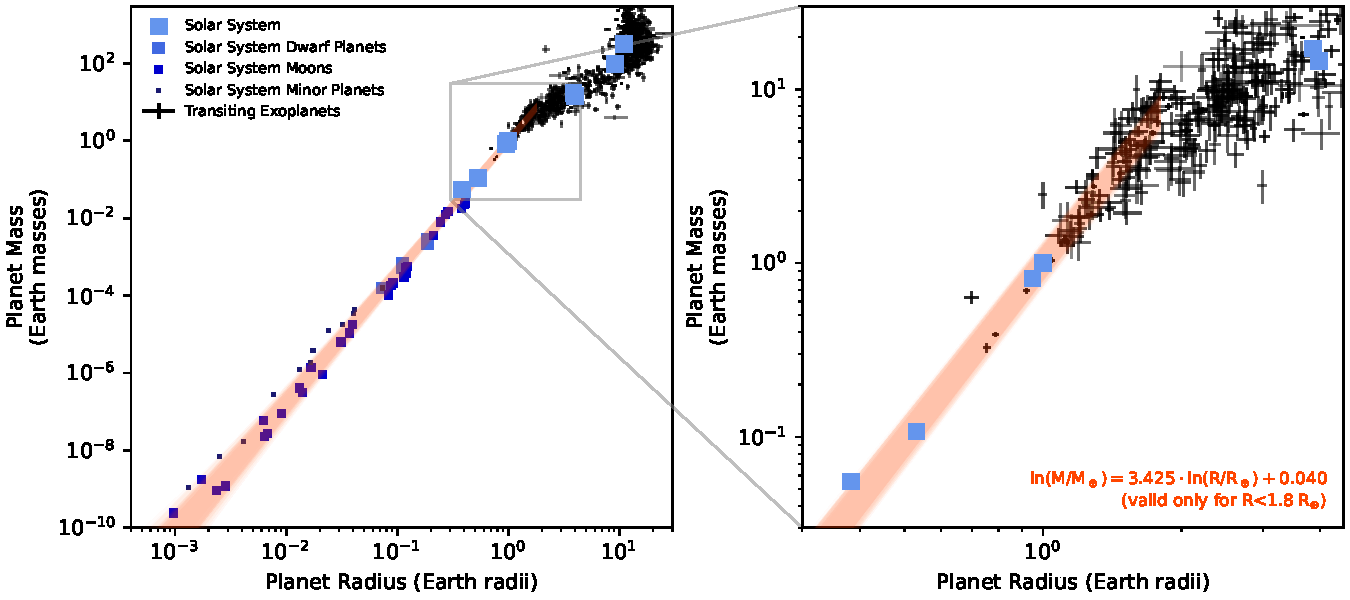
\includegraphics[width=\textwidth]{mass-radius-relation-for-rocky-planets}
\caption{To determine escape velocities for objects without measured masses, we derive an empirical mass-radius relationship from exoplanets (errorbars) and Solar System objects (squares). We use this relation, valid for rocky planets up to $1.8\rm{R}_\earth$, to estimate planet masses and uncertainties that incorporate the intrinsic scatter on the relation, the uncertainties on the model parameters, and uncertainties on the planet radii (\href{https://github.com/zkbt/shoreline/blob/main/notebooks/fit-mass-radius-relation.ipynb}{\texttt{</>}}).
}
\label{f:mass-radius}
\end{figure*}

\subsection{What planets do we label as having atmospheres?}

% We label planets (\href{https://github.com/zkbt/shoreline/blob/main/notebooks/curate-and-label-planets.ipynb}{\texttt{</>}}) as having an atmosphere ($A_{\sf i} = 1$) or not  ($A_{\sf i} = 0$), focusing on two subsamples of the exoplanet and Solar System population. 
To include in our probabilistic fit we label planets (\href{https://github.com/zkbt/shoreline/blob/main/notebooks/curate-and-label-planets.ipynb}{\texttt{</>}}) as having an atmosphere ($A_{\sf i} = 1$) or not ($A_{\sf i} = 0$). Planets with inconclusive or unmeasured atmospheres remain unlabeled ($A_{\sf i} = ?$) and are excluded from the fit. We focus on two subsamples of the exoplanet and Solar System population: a general \textbf{any atmosphere} sample and more specific \textbf{warm CO$_{2}$ atmosphere} subsample. In both cases, to simplify the analysis, we exclude planets with quoted ages younger than 500 Myr, to minimize having to imagine the future states of still rapidly evolving planets \citep{lopezUnderstandingMassRadiusRelation2014a, chenEvolutionaryAnalysisGaseous2016b,  thaoFeatherweightGiantUnraveling2024b}. 

For our {\bf any atmosphere} sample, we are generous in what we call ``having an atmosphere" ($A_{\sf i} = 1$), as in ZC17. For Solar System bodies, we include all major planets (everything except Mercury) and moons (Titan) with atmospheric surface pressures $>10^{-6}$ bar. We include outer Solar System moons or dwarf planets that have managed to retain significant volatile reservoirs \citep{schallerVolatileLossRetention2007}, either as seasonally sublimating atmospheres and/or substantial global N$_2$ and CH$_4$ volatile deposits on their surfaces: Triton, Pluto, Makemake, Eris \citep{youngStructureCompositionPlutos2018, sicardyConstraintsEvolutionTriton2024, grundyModerateRatiosMethane2024}. We label all other Solar System objects as $A_{\sf i} = 0$.

For exoplanets, planets larger than $2.2 \rm {R_\earth}$ are very difficult to explain with pure rocky compositions \citep{rogersMost16Earthradius2015b, zengNewPerspectivesExoplanet2021, rogersMostSuperEarthsHave2025}, so we label all planets 
with radii more than 1$\sigma$ over this limit as requiring atmospheres (or significant icy volatiles) to explain their low densities $A_{\sf i} = 1$. Many planets smaller than $2.0 \rm {R_\earth}$ have atmospheres too, but we apply labels only to those with direct atmosphere measurements, as follows.

We apply $A_{\sf i} = 1$ to one rocky planet with evidence for an atmosphere. 55 Cnc e shows variable JWST eclipse spectra suggesting a (potentially stochastically outgassed) CO/CO$_2$ atmosphere \citep{huSecondaryAtmosphereRocky2024, patelSecondaryAtmosphereRocky2024}. 

We apply $A_{\sf i} = 0$ to these rocky planets with eclipse observations of hot daysides that strongly suggest low albedos and poor global heat recirculation inconsistent with thick atmospheres \citep[see][]{kollIdentifyingCandidateAtmospheres2019c, mansfieldIdentifyingAtmospheresRocky2019b}. LHS 3844b, Gl 367b, TOI-1685b have a deep eclipses, symmetric phase curves, and dark night sides \citep{kreidbergAbsenceThickAtmosphere2019a, zhangGJ367bDark2024, luqueDarkBareRock2024}. GJ 1252b, TOI-1468b, LHS 1140c have deep photometric eclipses \citep{crossfieldGJ1252bHot2022, meiervaldesHotRocksSurvey2025, fortuneHotRocksSurvey2025a}, and
Gl 486b, GJ 1132b, and LTT 1445Ab have deep spectroscopic eclipses \citep{weinermansfieldNoThickAtmosphere2024, xueJWSTThermalEmission2024a, wachiraphanThermalEmissionSpectrum2025a}. We caution that our labeling these exoplanets as $A_{\sf i} = 0$ does {\em not} mean planets necessarily have no atmosphere at all; for tidally locked planets, a JWST measurement of hot dayside emission might only constrain the atmospheric pressure on an individual planet to less than about 10 bar \citep{kollScalingAtmosphericHeat2022}, really saying simply that we have not detected a very thick Venus-like atmosphere.

We leave the following notable planets unlabeled ($A_{\sf i} = ?$), meaning they are ignored from the probabilistic fit, even if there have been suggestions they lack atmospheres. 
Kepler-10b and Kepler-78b have symmetric phase curves from Kepler, but with only the optical bandpass their deep eclipses are degenerate between reflected and thermal light, thus complicating atmospheric inferences \citep{sanchis-ojedaTransitsOccultationsEarthsized2013, estevesChangingPhasesAlien2015a, huSemianalyticalModelVisiblewavelength2015, singhProbingKeplersHottest2022}. K2-141 shows a K2 + Spitzer phase curve suggesting a high albedo or hot inversion layer, but whether an atmosphere is absolutely required remains uncertain \citep{singhProbingKeplersHottest2022, ziebaK2SpitzerPhase2022}. LHS 1478b and TOI-431b appear to have a shallow thermal eclipses, but more data are needed to rule out systematics \citep{augustHotRocksSurvey2025, monaghanLow45Mm2025a}. TRAPPIST-1b and TRAPPIST-1c show deep MIRI eclipses implying hot day sides \citep{greeneThermalEmissionEarthsized2023, ihConstrainingThicknessTRAPPIST12023, ziebaNoThickCarbon2023, ducrotCombinedAnalysis1282025} and no obvious planetary transmission spectrum features \citep{limAtmosphericReconnaissanceTRAPPIST12023, radicaPromisePerilStellar2025, rathckeStellarContaminationCorrection2025}, but systemic stellar uncertainties leave the system still slightly ambiguous \citep{howardCharacterizingNearinfraredSpectra2023, rackhamRobustCorrectionsStellar2024,  fauchezStellarModelsAlso2025}. %LTT 1445Ab has a deep MIRI/LRS eclipse implying a hot dayside \citep{wachiraphanThermalEmissionSpectrum2025a}, but with the promise that it and LTT 1445Ac \citep{passHSTWFC3Light2023} will soon be observed at 15 $\mu$m in the Rocky Worlds program\footnote{\href{https://rockyworlds.stsci.edu/rw-website-targets.html}{rockyworlds.stsci.edu/rw-website-targets.html}} we leave it ambiguous for now. 
L 98-59 b's transmission spectrum may show tentative evidence of SO$_2$ \citep[possibly from tidally-heated volcanism;][] {seligmanPotentialMeltingExtrasolar2024} but is also consistent with featureless \citep{bello-arufeEvidenceVolcanicAtmosphere2025b}, so we leave it unlabeled. Otherwise, transmission spectra have not yet conclusively identified nor ruled out any rocky planet atmospheres due to degeneracies with clouds \citep{lustig-yaegerMirageCosmicShoreline2019} and/or stellar contamination \citep{mayDoubleTroubleTwo2023, moranHighTideRiptide2023}; we leave transmission spectroscopy-based non-detections as $A_{\sf i} = ?$.

Four targets are already planned for Rocky Worlds. GJ 3929b \citep{beardGJ3929Highprecision2022, kemmerDiscoveryMassMeasurement2022} and LTT 1445Ac \citep[][]{wintersSecondPlanetTransiting2022, passHSTWFC3Light2023, laviePlanetarySystemLTT2023} have no atmosphere measurements and are both $A_{\sf i}=?$. LHS 1140b \citep{dittmannTemperateRockySuperEarth2017c, mentSecondTerrestrialPlanet2019c} may show hints of an atmosphere in transmission \citep{cadieuxTransmissionSpectroscopyHabitable2024}, but we keep it as $A_{\sf i}=?$ for now. LTT 1445Ab is labeled here as $A_{\sf i}=0$ based the lack of a thick ($>10$ bar) atmosphere (see above), but Rocky Worlds' 15$\mu$m photometry should be sensitive to much more tenuous CO$_2$ atmospheres and could in the future flip it to $A_{\sf i}=1$. 

For our {\bf warm CO$_2$ atmosphere} sample, we restrict the above sample to planets with zero-albedo equilibrium temperatures cool enough to have a solid surface \citep[$< 1700\mathrm{K}$;][]{boukareDeepTwophaseHemispherical2022}, trying to avoid magma oceans that might tilt a cosmic shoreline by providing direct contact with a much deeper volatile reservoir \citep[see][]{huSecondaryAtmosphereRocky2024}. We also limit to temperatures warm enough for CO$_2$ to be gaseous ($>$194 K, CO$_2$ saturation vapor pressure of 1 bar; \citealt{pierrehumbertPrinciplesPlanetaryClimate2010}), coinciding approximately with the outer edge of the habitable zone \citep[where CO$_2$ can no longer provide greenhouse warming because it condenses out of the atmosphere;][]{kopparapuHabitableZonesMainsequence2013}. We focus on CO$_2$ and O$_2$ (which condenses at even colder temperatures) as likely major constituents of temperate atmospheres distilled by near-complete atmospheric erosion \citep{hamanoEmergenceTwoTypes2013a, lugerExtremeWaterLoss2015, schaeferPredictionsAtmosphericComposition2016c,  krissansen-tottonErosionLargePrimary2024}. Venus (92 bar) and Mars ($0.004-0.009$ bar) are both about 95\% CO$_2$ \citep{loddersPlanetaryScientistsCompanion1998}, and Earth too would likely have about 100 bars of atmospheric CO$_2$ (swamping our 1 bar of N$_2$ + O$_2$; \citealt{ingersollPlanetaryClimates2013}) if not for the presence of H$_2$O continually raining down, dissolving atmospheric CO$_2$, and locking it away into solid carbonates \citep{walkerNegativeFeedbackMechanism1981, lecuyerComparisonCarbonNitrogen2000, wordsworthAtmospheresRockyExoplanets2022, hansenDetectingAtmosphericCO22025}. Earth preserves its H$_2$O (and thus keeps our CO$_2$ trapped in limestone deposits) only because water precipitates before it reaches the upper atmosphere, where it would be dissociated by UV radiation and its H atoms lost to space. On warm Venus, the runaway greenhouse process \citep{komabayasi1ChengFen2XiangXinoDaQiQuantoShuiQuanwoYousuruJiaXiangDenaHuoXinggaYiDingnoTaiYangGuangXiadetoriuruBuLianSoknaPingHengWenDunituite1ChengFen2XiangXinoDaQiQuantoShuiQuanwoYousuruJiaXiangDenaHuoXinggaYiDingnoTaiYangGuangXiadetoriuruBuLianSoknaPingHengWenDunituiteDiscreteEquilibriumTemperatures1967, ingersollRunawayGreenhouseHistory1969} vaporizes water and drives it inevitably to the upper atmosphere, where its H escapes \citep{hamanoEmergenceTwoTypes2013a, leconteIncreasedInsolationThreshold2013, wordsworthWaterLossTerrestrial2013}. On cold Mars, hydrogen has also been preferentially lost \citep{jakoskyLossMartianAtmosphere2018}, with modern escape largely driven by dust dynamics carrying frozen water up to high altitudes \citep{chaffinMartianWaterLoss2021}. CO$_2$ (possibly mixed with O$_2$) atmospheres are also particular detectable for exoplanets with JWST, especially with Rocky Worlds' use of MIRI filter photometry centered on the strong 15 $\mu$m CO$_2$ absorption band \citep{morleyObservingAtmospheresKnown2017b, ihConstrainingThicknessTRAPPIST12023}. 

The {\bf any atmosphere} sample contains 965 $A_{\sf i} = 1$ and 42 $A_{\sf i} = 0$ planets, and the {\bf warm CO$_2$} sample contains 538 $A_{\sf i} = 1$ and 12 $A_{\sf i} = 0$ planets. By comparing the broader {\bf any} sample to the smaller zoomed-in {\bf warm CO$_2$} sample, we can test for evidence of the shoreline changing from the global scale (all planets, all volatiles) to the local scale (temperate rocky planets). 



\section{Fitting a Cosmic Shoreline}
\label{s:fitting} 

We construct a generative model that tries to explain the atmosphere labels $A_{\sf i}$ for planet $i$ using the predictors $f_{\sf i}$, $v_{\sf esc, i}$, $L_{\sf \star, i}$. We first define a cosmic shoreline flux $f_{\sf shoreline}$ for escape velocity $v_{\sf esc}$ and stellar luminosity $L_\star$ with the power law expression

\begin{equation}
\label{e:f_shoreline}
f_{\sf shoreline} = f_{\sf 0} \left(\frac{v_{\sf esc}}{v_{\sf esc, \oplus}}\right)^p\left(\frac{L_\star}{L_\sun}\right)^q
\end{equation}
where $f_{\sf 0}$, $p$, and $q$ are model parameters, $v_{\sf esc, \earth} = 11.18$ km/s is Earth's escape velocity, and $L_\sun = 3.828 \times 10^{26}$ W is the Sun's luminosity. We compare all fluxes to Earth's average bolometric flux $f_\earth = L_\sun/(4\pi a)^2 = 1361 \mathrm{W/m^2}$. This power law log transforms to a linear plane
\begin{equation}
\label{e:log_f_shoreline}
 \log_{10} \left(\frac{f_{\sf shoreline}}{f_\earth}\right)  =  \log_{10} \left(\frac{f_{\sf 0}}{f_\earth}\right)  + p \cdot  \log_{10} \left(\frac{v_{\sf esc}}{v_{\sf esc, \oplus}}\right) + q \cdot  \log_{10} \left(\frac{L_\star}{L_\sun}\right).
\end{equation}
We define a distance from this shoreline in log-flux as 
\begin{equation}
\label{e:delta}
\Delta =  \log_{10} \left(\frac{f_{\sf }}{f_\earth}\right) - \log_{10}\left(\frac{f_{\sf shoreline}}{f_\earth}\right) = \log_{10}\left(\frac{f}{f_{\sf shoreline}}\right)
\end{equation}
which is similar to the Atmosphere Retention Metric from \citet{passRecedingCosmicShoreline2025}. We use this distance to describe the probability of each planet having an atmosphere with the logistic function \citep[see][]{ivezicStatisticsDataMining2020} as
\begin{equation}
p_{\sf i} = P(A_{\sf i} = 1 | \mathbf{x}_{\sf i}, \boldsymbol{\theta} ) = \frac{1}{1+e^{\Delta_{\sf i}/w}}
\label{e:p_i}
\end{equation}
where $\mathbf{x}_{\sf i} = [\log_{10}(f_{\sf i}/f_\earth), \log_{10} (v_{\sf esc, i}/v_{\sf esc, \earth}), \log_{10} (L_{\sf \star, i}/L_\sun)]$ are the predictors for each datum and $\boldsymbol{\theta} = [f_{\sf 0}, p, q, w]$ are the model parameters. This logistic function smoothly transitions from 1 when $f$ is below the shoreline to 0 above, with the width parameter $w$ describing the fuzziness of the shoreline, how quickly in $\log_{10} (f/f_\earth)$ planets change from mostly having atmospheres to mostly not. The likelihood of the data ensemble $\mathbf{A}$ can be calculated by multiplying $p_{\sf i}^{A_{\sf i}}$ (= how well did we predict the presence of an atmosphere) by $(1-p_{\sf i})^{1-A_{\sf i}}$ (= how well did we predict the absence of an atmosphere) across all data points (a Bernoulli distribution):

\begin{equation}
P(\mathbf{A} | \boldsymbol{\theta}) = \prod_{i=1}^{N} p_{\sf i}^{A_{\sf i}} \cdot (1-p_{\sf i})^{1-A_{\sf i}}
\end{equation} 
This likelihood $P(\mathbf{A} | \boldsymbol{\theta})$
 and a prior $P(\boldsymbol{\theta})$ together determine the posterior probability $P(\boldsymbol{\theta} | \mathbf{A}) = P(\mathbf{A} | \boldsymbol{\theta}) P(\boldsymbol{\theta})$. For $f_{\sf 0}$, we adopt an uninformative uniform prior on $\log_{10} (f_{\sf 0}/f_\earth)$. For $p$, and $q$, we adopt the uninformative prior $P(\boldsymbol{\theta}) \propto (1+p^2)^{-3/2}\cdot (1+q^2)^{-3/2}$, which avoids the infinitely growing prior space toward high slope values and effectively represents a uniform prior on the rotation angle of the slopes in log space \citep[see][]{vanderplasFrequentismBayesianismPythondriven2014a}. For $w$, we adopt a uniform prior of $-6 > \ln w > 2$,  spanning $0.0024~\mathrm{dex} < w < 7.4~\mathrm{dex}$, or from a 0.57\% change in $f$ at the narrowest to a factor of $2.5\times10^7$ change in $f$ at the widest; practically we find that allowing narrower widths than this can reveal sharp discontinuities that become difficult to sample. 

To account for measurement uncertainties on the predictors, the expression for $p_{\sf i}$ in Equation \ref{e:p_i} should be marginalized over the distribution of true (unknown) values for each planet's $\mathbf{x}_{\sf i}$. While this marginalization can sometimes be done analytically (as in the mass-radius fit in \S\ref{f:mass-radius}), we were unable to find a simple analytic expression and instead relied on the {\em remarkable} efficiency of \texttt{numpyro}'s NUTS sampler to do this marginalization numerically. We introduced three parameters for {\em each} datapoint (1,007 planets for {\bf any}, 550 planets for {\bf warm CO$_2$}) to represent the true values of $\mathbf{x}_{\sf i}$ with normal priors centered on the measured values and the uncertainties as their widths, and we sampled these alongside the 4 parameters $\boldsymbol{\theta}$. 

We used \texttt{numpyro} with NUTS to sample from this posterior, running 4 chains with 5,000 warm-up steps and 50,000 samples each, always achieving a Gelman-Rubin statistic of 1.0 across the chains and usually achieving an effective sample size always (and sometimes much) larger than 1,000 (\href{https://github.com/zkbt/shoreline/blob/main/notebooks/fit-one-shoreline.ipynb}{\texttt{</>}}). Even with the thousands of hyperparameters we use to marginalize over measurement uncertainties, this sampling takes only a few minutes on a modern MacBook Pro. We repeat these fits, with and without uncertainties, across various subsamples of the data (\href{https://github.com/zkbt/shoreline/blob/main/notebooks/fit-many-shorelines.ipynb}{\texttt{</>}}).

\begin{figure*}[ht!]
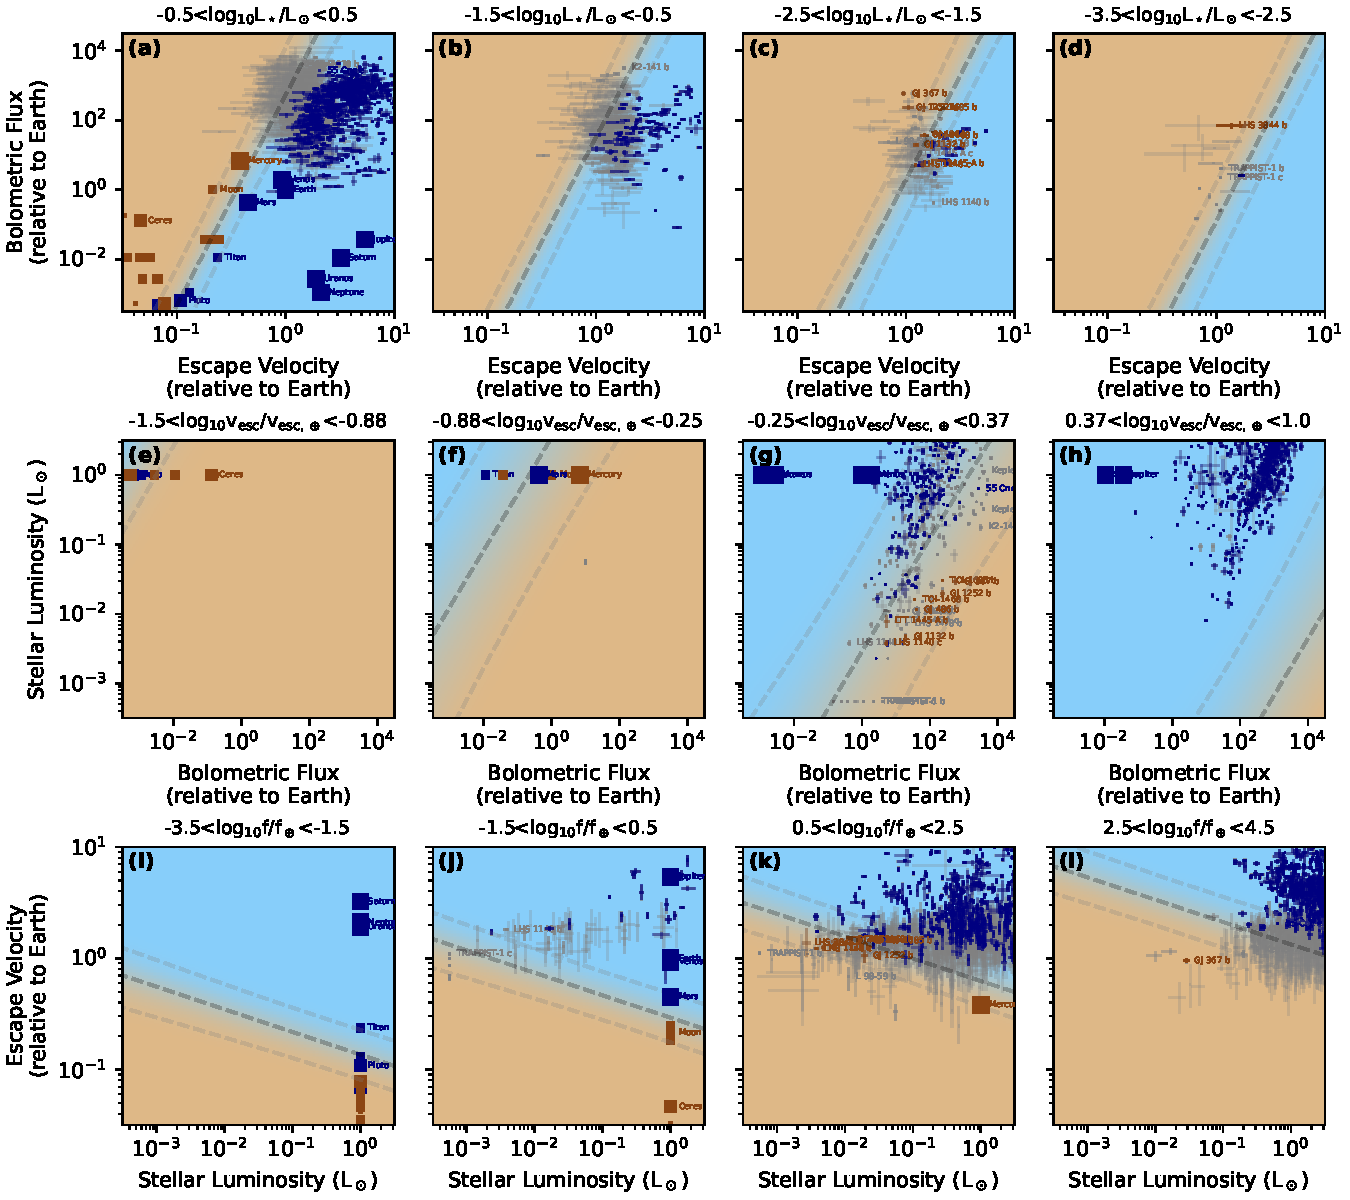
\includegraphics[width=\textwidth]{grid-of-shorelines-any.pdf}
\caption{A cosmic shoreline dividing exoplanets (errorbars) and Solar System planets (squares) with {\bf any} type of atmosphere or global surface volatiles (blue symbols, $A_{\sf{i}}=1$) from those without (brown symbols, $A_{\sf{i}}=0$). Planets without definitive atmosphere constraints are shown for context (gray symbols, $A_{\sf{i}}=?$). The shoreline defines a plane in the 3D space of ($f$, $v_{\sf esc}$, $L$); each row shows slices that consider a narrow range of stellar luminosity (top), planet escape velocity (middle), and planet flux (bottom). Background colors indicate the modeled probability of an atmosphere at each location (sandy brown for $p_{\sf i} = 0$, water blue for $p_{\sf i}$ = 1), accounting for the intrinsic width of the shoreline and marginalizing over the parameter uncertainties and the width of the slice; contours (dashed lines) highlight atmosphere probabilities of 5\%, 50\%, 95\% (\href{https://github.com/zkbt/shoreline/blob/main/notebooks/plot-shorelines.ipynb}{\texttt{</>}}).}
\label{f:shoreline-any}
\end{figure*}


\section{Shorelines in 3D}
\label{s:shorelines}

\subsection{{\bf any} atmosphere shoreline}
Figure \ref{f:shoreline-any} shows the inferred shoreline model for the {\bf any} atmosphere subset, representing the question of whether a planet has any type of atmosphere or volatile reservoir across a broad range of flux, similar to ZC17. Because the probability of an atmosphere $A$ is a function in a 3D volume, it can be a little tricky to visualize. We display this 3D volume in slices: each row holds one dimension fixed to a narrow range and visualizes the other two dimensions on the $x$ and $y$ axes, and each column displays a different range of values for the fixed dimension. The background color shows the modeled probability of an atmosphere at each $(x, y)$ location in each slice, marginalized (= integrated, see \citealt{hoggDataAnalysisRecipes2010a, siviaDataAnalysisBayesian2011, vanderplasFrequentismBayesianismPythondriven2014a, ivezicStatisticsDataMining2020}) over both the width of the slice and the uncertainties on the model parameters. Even for infinitely thin slices with no parameter uncertainties the transition would still appear fuzzy due to the intrinsic width $w$ (see Equation \ref{e:p_i}). 



The top row (a-d) of Figure \ref{f:shoreline-any} holds $L_\star$ as the fixed dimension, decreasing from solar type host stars on the left to the latest possible M dwarf stars on the right. The centers of these luminosity ranges (1$L_\sun$, 0.1$L_\sun$, 0.01$L_\sun$, 0.001$L_\sun$) correspond to main-sequence spectral types (G2, K7, M3.5, and M6) according to the \citet{pecautINTRINSICCOLORSTEMPERATURES2013} sequence. Panel (a) shows $v_{\sf esc}$ and bolometric flux $f$ for both Solar System objects (all with $L = 1.0L_\sun$) and exoplanets with host stars within a factor of $\sqrt{10}$ of the Sun's luminosity; it is the closest analog to Figure 1 from ZC17, which shows similar quantities but without the restriction on exoplanet host star type. The shoreline in this row has a slope of $p$ (see Equation \ref{e:log_f_shoreline}) and reading from left to right appears to recede \citep[to borrow a visual metaphor from][]{passRecedingCosmicShoreline2025} down and to the right, with the bolometric threshold $f_{\sf shoreline}$ decreasing at fixed $v_{\sf esc}$ toward lower luminosity stars. 

The middle row (e-h) shows shoreline slices for different fixed $v_{\sf esc}$, increasing from tiny low-mass dwarf planets on the left to gas giants on the right. Only Solar System objects are known at low $v_{\sf esc}$ (e), but for Earth-like $v_{\sf esc}$ values (g) exoplanet atmosphere data become available either as radii large enough to require volatiles or as rocky planets with JWST hot dayside brightness temperatures disfavoring thick atmospheres. In these slices the visible slope is $1/q$, with cooler less luminous stars having lower maximum allowable flux levels $f_{\sf shoreline}$ for atmospheres to survive. 

The bottom row (i-l) shows the shoreline for different fixed $f$, increasing from the cold outer regions of the Solar System on the left to the very hottest exoplanets on the right. The slope of the shoreline in this projection is $-q/p$ and indicates a larger $v_{\sf esc}$ is necessary in order for lower $L_\star$ hosts to permit atmospheres. For temperate planets (j), if we imagine shrinking the host star luminosity while keeping $f$ constant, Mars-sized planets would be unable to retain atmospheres around stars less luminous than $0.1~L_\sun$, and Earth/Venus-size planets would likely lose atmospheres somewhere between $10^{-3} - 10^{-2}~L_\sun$.


\begin{figure*}[ht!]
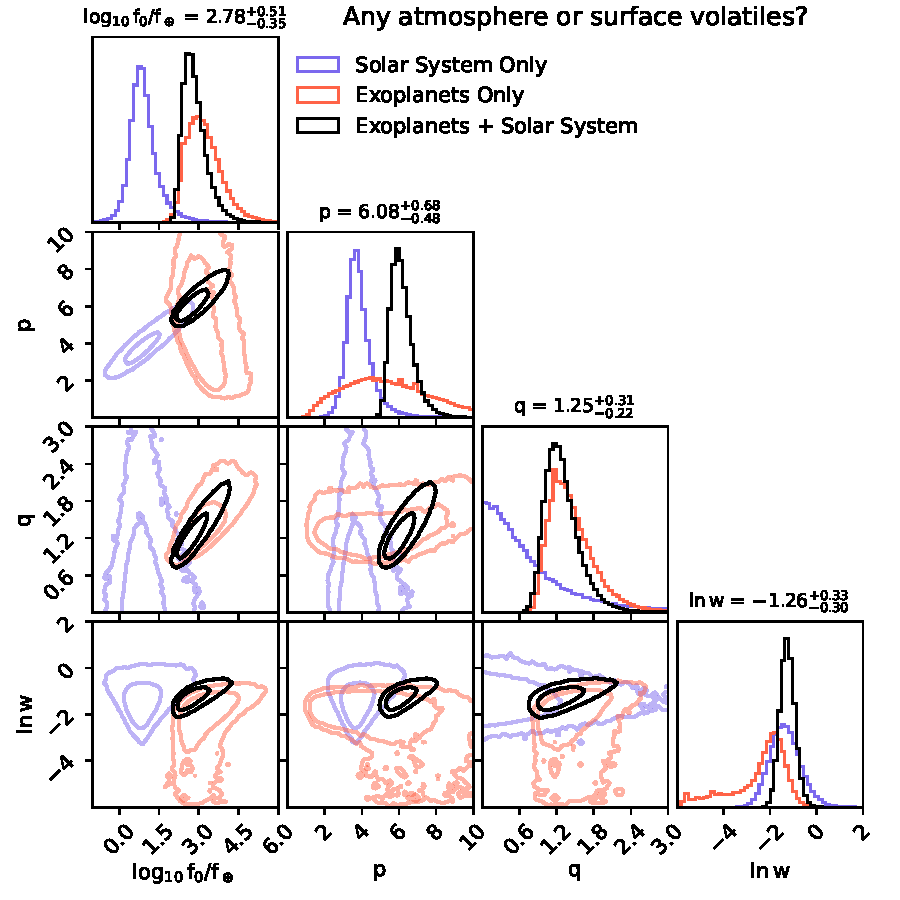
\includegraphics[width=\textwidth]{posteriors-any.pdf}
\caption{Cosmic shoreline parameter posterior probabilities for {\bf any} atmosphere or surface volatiles, corresponding to data in Figure \ref{f:shoreline-any}. Panels show marginalized 1D histograms (diagonal) and marginalized 2D distributions (off-diagonal) with contours that enclose 68.3\% and 95.4\% probability. Titles along the diagonal show confidence intervals for the exoplanets + Solar System joint fit. The model parameters define a shoreline via $\log_{10} (f_{\rm shoreline}/f_\earth) = \log_{10} (f_{\sf 0}/f_\earth) + p \log_{10} (v_{\sf esc}/v_{\sf esc, \earth}) + q \log_{10} (L_\star/L_\sun)$, with $w$ representing the logistic width parameter setting the fuzziness of the shoreline  (\href{https://github.com/zkbt/shoreline/blob/main/notebooks/print-and-visualize-posteriors.ipynb}{\texttt{</>}}).}
\label{f:posteriors-any}
\end{figure*}

Figure \ref{f:posteriors-any} shows posterior probability distribution for shoreline parameters considering {\bf any} kind of atmosphere or surface volatiles. In addition to the main fit including all planets together, we also show what we might learn from just Solar System or just exoplanets each by themselves. We compare these posteriors with \texttt{corner.py} \citep{foreman-mackeyCornerpyScatterplotMatrices2016}, with contours in each 2D panel that enclose 68.3\% and 95.4\% of the probability marginalized over other parameters. 

We find the intercept to be $\log_{10}{f_{\sf 0}} = \allanyTruelogfo$, meaning that an Earth-size planet orbiting a Sun-like star should on average be able to retain an atmosphere with flux levels $f/f_\earth$ up to about $10^{\allanyTruelogfojustvalue} = \allanyTruefojustvalue$. If we moved Earth inward toward the Sun, hydrogen and the hope of habitability would be lost long before this limit, likely leaving heavily oxidized CO$_2$/O$_2$ atmospheres.

The escape velocity slope $p = \allanyTruep$ is marginally steeper than $p=4$ chosen by ZC17 and means that a factor of $10\times$ increase in $v_{\sf esc}$ causes the critical flux $f_{\sf shoreline}$ to move up by $10^{\allanyTruepjustvalue}$. Notably, for Solar System planets alone we find $p = \solaranyTruep$ and for exoplanets alone we find $p = \exoanyTruep$ (both consistent with $p=4$), so the higher joint slope reflects a compromise where these two different samples that mostly occupy different regions of parameter space can agree.

The stellar luminosity slope $q = \allanyTrueq$ means that if we decrease the luminosity of the host star by $10\times$, the maximum flux that permits atmospheres $f_{\sf shoreline}$ decreases by a factor $10^{\allanyTrueqjustvalue}$. This is steep! If we take $f_{\sf hz} = f_\earth$ as a crude approximation for the habitable zone (neglecting the important dependence on the stellar spectrum; \citealt{kopparapuHabitableZonesMainsequence2013}), this fit implies $f_{\sf shoreline} < f_{\sf hz}$ for stars less luminous than $\log_{10} (L_\star/L_\sun) = \allanyTruelogLnohz$ or $L_\star/L_\sun = \allanyTrueLnohz$, corresponding to M4V spectral type \citep{pecautINTRINSICCOLORSTEMPERATURES2013} or  $0.25 \mathrm{M_\sun}$ mass \citep{, pinedaMdwarfUltravioletSpectroscopic2021}. Cast in terms of semimajor axis $a$, the habitable zone distance necessarily shrinks toward smaller stars as $a_{\sf hz} \propto L_\star^{1/2}$ \citep[generally making them easier to observe;][]{blakeNearInfraredMonitoringUltracool2008, nutzmanDesignConsiderationsGroundBased2008a}. The shoreline distance scales as $a_{\sf shoreline} \propto L_\star^{(1-q)/2}$, so $q > 1$ means that $a_{\sf shoreline}$ grows larger toward smaller stars, with ominous prospects for atmospheric retention around the coolest stars.

The intrinsic width of the shoreline $\ln w = \allanyTruelnw$, or $w = \allanyTruew~\mathrm{dex}$, means than if $f$ increases by a factor of $10^{\allanyTruewjustvalue}$ above $f_{\sf shoreline}$ then the probability of an atmosphere drops from $50\%$ to $1/(1 + e^{1}) = 27\%$ (Equation \ref{e:p_i}). To translate into more familiar probabilities from a normal distribution, the chance of having an atmosphere drops to 16\% (1$\sigma$) and 5\% (2$\sigma$) at $1.7w$ and $2.9w$, respectively. The transition from atmospheres being 95\% likely to only 5\% likely spans $w_{95} = 5.89w = \allanyTruewninetyfivejustvalue~\mathrm{dex}$ or a factor of $\allanyTruewninetyfiveasfluxfactorjustvalue \times$ in flux (\href{https://github.com/zkbt/shoreline/blob/main/notebooks/logistic-probabilities.ipynb}{\texttt{</>}}), seen as the blending of colors in Figure \ref{f:shoreline-any}. 




\subsection{{\bf warm CO$_2$} atmosphere shoreline}

Figure \ref{f:shoreline-CO2} shows the shoreline inferred for the zoomed-in {\bf warm CO$_2$} sample of planets, including only those with equilibrium temperatures warm enough for CO$_2$ to remain in gaseous form and cool enough to not necessitate a dayside magma ocean. Focusing on the local geography of the cosmic shoreline more relevant to JWST, the most important differences are (a) the absence of the ultrahot atmosphere 55 Cnc e at high $f$ and (b) the lack of small icy objects to anchor the slope down at low $f$. We see the same qualitative story as before: less luminous stars create harsher environments for planetary atmospheres. 

\begin{figure*}[ht!]
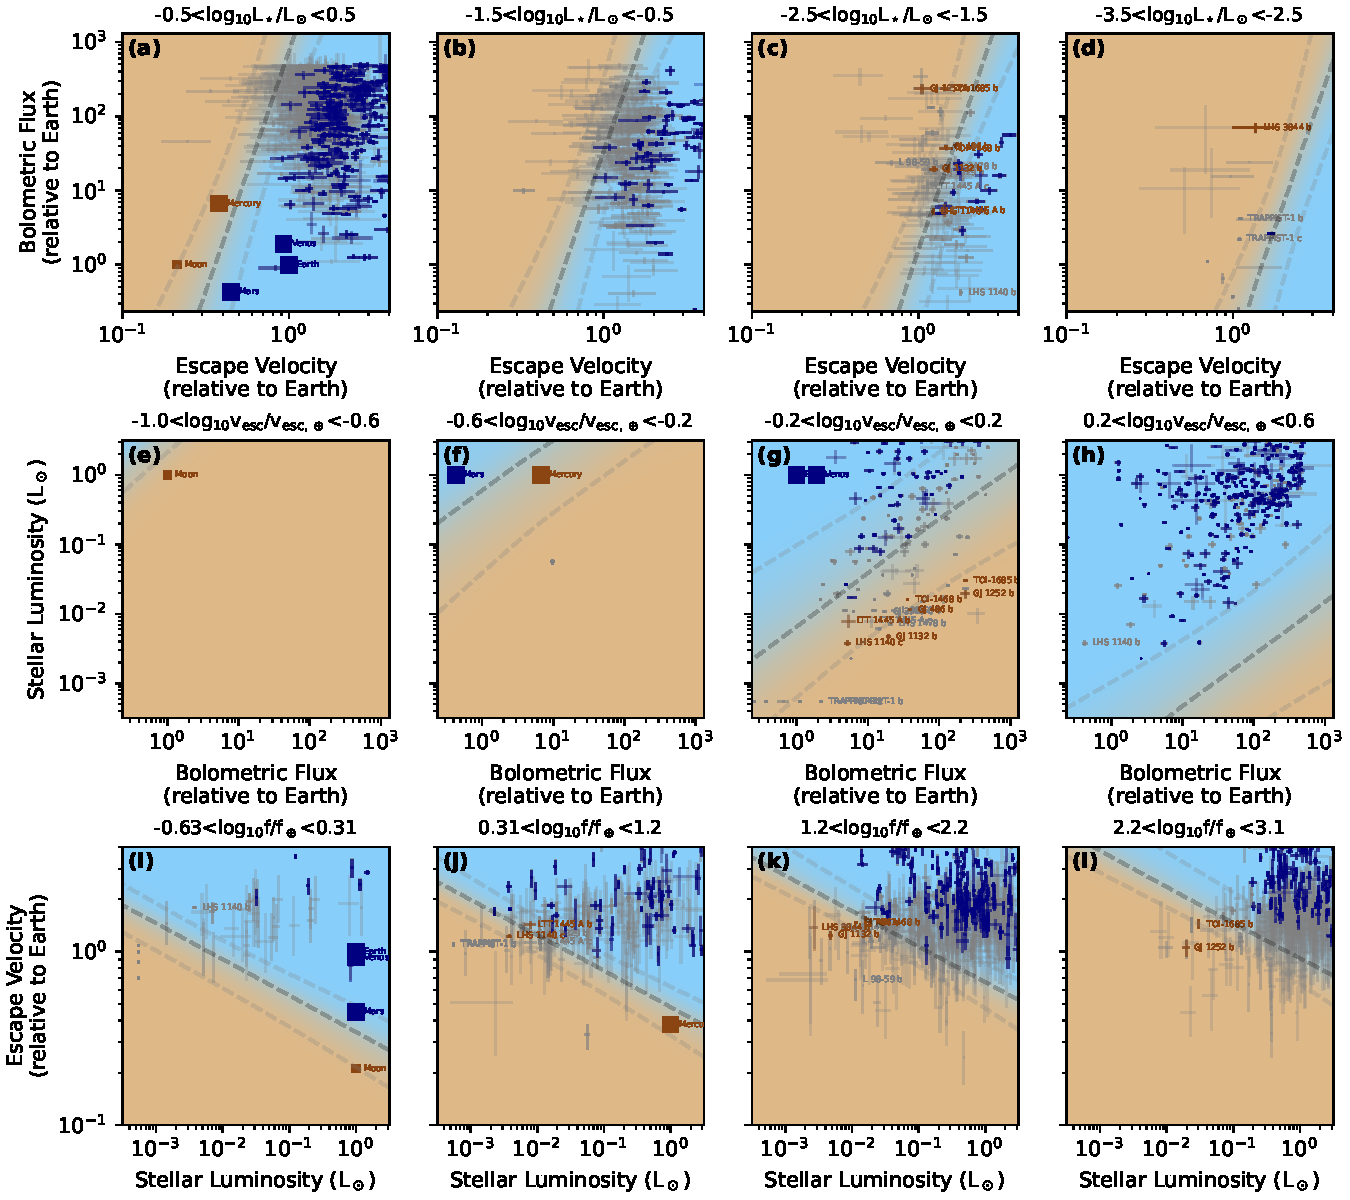
\includegraphics[width=\textwidth]{grid-of-shorelines-CO2.pdf}
\caption{A cosmic shoreline exactly as in Figure \ref{f:shoreline-any}, but specifically targeting $\rm{CO}_2$-dominated atmospheres on planets with equilibrium temperatures warm enough $\rm{CO_2}$ to exist as a gas (${\rm T_{CO_2}}= 194 \mathrm{K}$) and cool enough that a global magma ocean is less likely (${\rm T_{magma}} = 1700 \mathrm{K}$). This more narrowly defined cosmic shoreline matters because $\rm CO_2$ is both likely in warm secondary atmospheres and relatively easier to detect for exoplanets in thermal emission with JWST (\href{https://github.com/zkbt/shoreline/blob/main/notebooks/plot-shorelines.ipynb}{\texttt{</>}}).}
\label{f:shoreline-CO2}
\end{figure*}

Figure \ref{f:posteriors-CO2} shows the {\bf warm CO$_2$} parameter posterior. We find $\log_{10} (f_{\sf 0}/f_\earth) = \allCOOTruelogfo$, $p = \allCOOTruep$, and $q = \allCOOTrueq$ for the shape of the shoreline, mostly consistent within uncertainties with the previous results. Figure \ref{f:posteriors-uncertainties} shows the joint fits for both samples, permitting more direct comparison between the two. Relative to the any atmosphere fits, the CO$_2$ parameter uncertainties are larger, probably due to the narrower range of fluxes providing leverage on the slope. Slopes nudge toward marginally shallower, but not significantly so. 

The biggest difference is $\ln w = \allCOOTruelnw$ or $w = \allCOOTruew$ dex being much lower for the narrower CO$_2$ sample, with a transition from 95\% to 5\% atmosphere probability spanning $w_{95} = \allCOOTruewninetyfivejustvalue$ dex or a factor of $\allCOOTruewninetyfiveasfluxfactorjustvalue\times$ in flux. One possibility is that the width $w$ on broad global scales is partially capturing unknown curvature or topography along the shoreline, and a lower $w$ in the zoomed-in sample might hint at the log-linear shoreline being a better local description on increasingly fine scales. Testing this hypothesis will require many more planets with reliable atmosphere labels. 

\begin{figure*}[ht!]
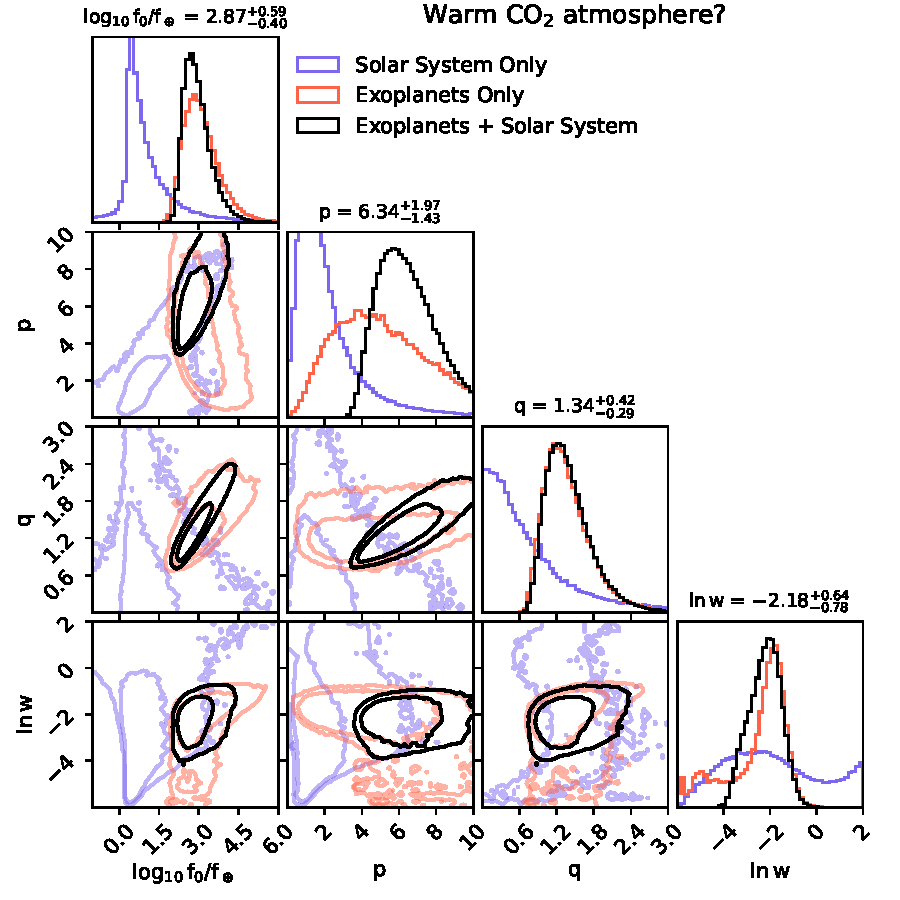
\includegraphics[width=\textwidth]{posteriors-CO2.pdf}

\caption{Cosmic shoreline parameter posterior probabilities for {\bf warm CO$_2$} atmosphere or surface volatiles, corresponding to data in Figure \ref{f:shoreline-CO2}. Panels show marginalized 1D histograms (diagonal) and marginalized 2D distributions (off-diagonal) with contours that enclose 68.3\% and 95.4\% probability. Titles along the diagonal show 68.3\% confidence intervals for the exoplanets + Solar System joint fit. The model parameters define a shoreline via $\log_{10} (f_{\rm shoreline}/f_\earth) = \log_{10} (f_{\sf 0}/f_\earth) + p \log_{10} (v_{\sf esc}/v_{\sf esc, \earth}) + q \log_{10} (L_\star/L_\sun)$, with $w$ representing the logistic width parameter setting the fuzziness of the shoreline (\href{https://github.com/zkbt/shoreline/blob/main/notebooks/print-and-visualize-posteriors.ipynb}{\texttt{</>}}).}
\label{f:posteriors-CO2}
\end{figure*}




\begin{figure*}[ht!]
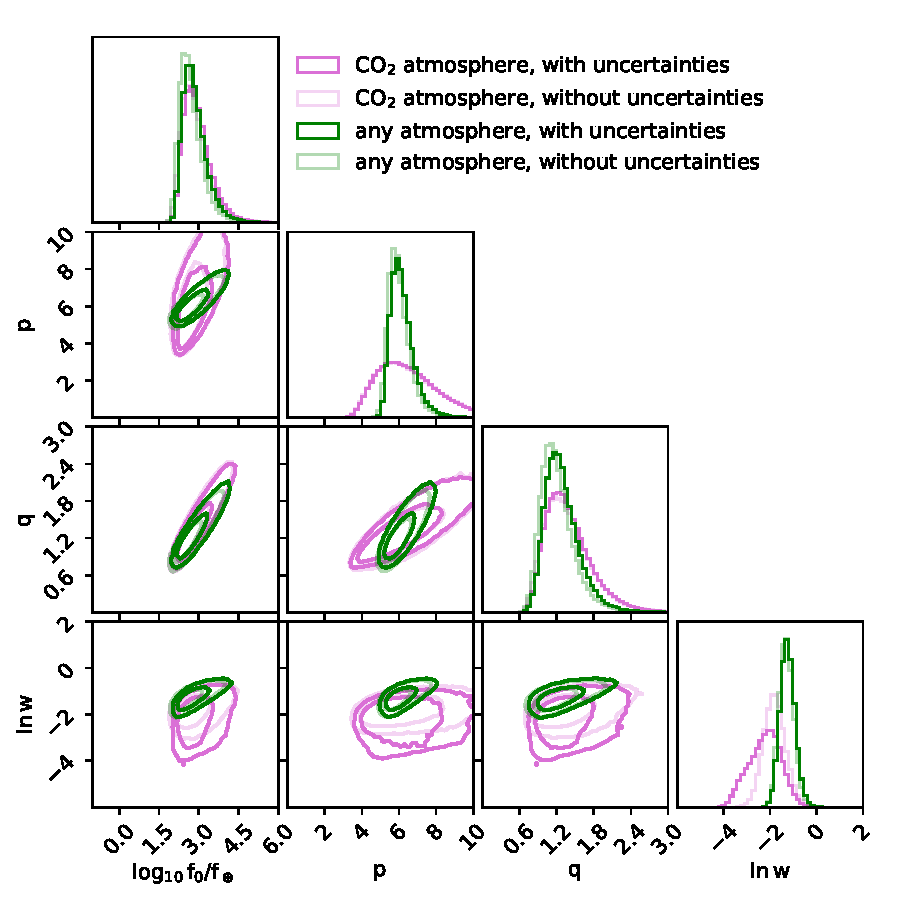
\includegraphics[width=\textwidth]{posteriors-with-and-without-uncertainties.pdf}
\caption{Posteriors inferred with (intense lines) and without (faint lines) accounting for uncertainties on planet properties ($f$, $v_{\sf esc}$, $L_\star$). Both types of atmosphere are shown, using exoplanet and Solar System data in all fits. Marginalizing over uncertainties broadens the possible intrinsic shoreline widths $w$ to lower values but does not significantly shift the shoreline shape parameters (\href{https://github.com/zkbt/shoreline/blob/main/notebooks/print-and-visualize-posteriors.ipynb}{\texttt{</>}}).}
\label{f:posteriors-uncertainties}
\end{figure*}





%For a star like TRAPPIST-1 at $\log_{10} (L_\star/L_\sun) = -3.26 \pm 0.01$ \citep{ducrotTRAPPIST1GlobalResults2020}, a value of $q=1.21$ implies the shoreline for an Earth-mass planet ($v_{\sf esc} = v_{\sf esc, \earth}$) occurs at $f_{shoreline} = 0.075 f_\earth$ or $a_{\sf shoreline} = 



\subsection{Sensitivity to Including Gas Giant Planets}
In these fits, we did not place upper limits on planet escape velocity or radius, allowing all giant planets to participate in sculpting the shoreline, as in ZC17. Hot Jupiters could potentially bias the shoreline slope, in that they might lose tens of Earth masses of atmosphere but still appear as $A_{\sf i} = 1$. We tested the sensitivity of the inferred shoreline to this concern by repeating the fits including only planets smaller than Neptune; we found no significant changes to the parameters. 

\subsection{Sensitivity to Planet Parameter Uncertainties}
We test the impact that measurement uncertainties on the predictors $v_{\sf esc}, f, L_\star$ have the inferred shoreline. Figure \ref{f:posteriors-uncertainties} shows parameter posteriors with and without including parameter uncertainties. Including them slightly broadens distributions and tends to allow for lower values of $w$, where disagreeing labels at fixed shoreline distance $\Delta_{\sf i}$ can be a little more explained by uncertainties on the predictors and require a little less intrinsic fuzziness. This is especially true for the warm CO$_2$ sample; with fewer planets, each planet's position relative to the shoreline matters more. Still, the differences are minor, likely because parameter uncertainties for most well-characterized planets are smaller than the intrinsic width $w$. 

\section{Physical Interpretation}
\label{s:physics}

Atmospheric loss is fundamentally a matter of energy balance: whatever energy a planet receives from its star (or still-cooling interior; see \citealt{guptaSculptingValleyRadius2019}), must either radiate away or be carried away in the gravitational potential energy of escaping gas \citep{lewisPlanetsTheirAtmospheres1984, chamberlainTheoryPlanetaryAtmospheres1987}. The incoming energy need not be radiative, with particles and fields in the stellar wind also driving loss, and moreso during coronal mass ejections \citep{lammerCoronalMassEjection2007, jakoskyMAVENObservationsResponse2015}. Modeling efforts beyond ZC17 have included various atmospheric sources and sinks to understand where atmospheres can or cannot flourish \citep{tianTHERMALESCAPESUPER2009,
lugerHabitableEvaporatedCores2015, 
owenEvaporationValleyKepler2017, 
wyattSusceptibilityPlanetaryAtmospheres2020, 
guptaCaughtActCorepowered2021,
chatterjeeNovelPhysicsEscaping2024, 
chinRolePlanetaryRadius2024a, 
giallucaImplicationsThermalHydrodynamic2024,
teixeiraCarbondeficientEvolutionTRAPPIST1c2024,
zengCosmicHydrogenIce2024,
vanlooverenAiryWorldsBarren2024,
vanlooverenHabitableZoneAtmosphere2025, 
leeCarvingEdgesRocky2025,
jiCosmicShorelineRevisited2025}. Here, we briefly try to contextualize the newly inferred shoreline parameters through the lens of hydrodynamic escape, as the most efficient path for atmospheric erosion in extreme environments where XUV heating can overwhelm infrared cooling in the tenuous upper atmosphere and drive fluid flows \citep{sekiyaDissipationRareGases1980, watsonDynamicsRapidlyEscaping1981}. 

For the flux slope $p$, we can consider a simplified model of energy-limited escape, where some fraction $\epsilon_{\sf esc}$ of incoming power from $f_{\sf XUV}$ radiation converts directly into gravitational potential energy of outflowing atmosphere \citep{watsonDynamicsRapidlyEscaping1981}, can be written as $\epsilon_{\sf esc} f_{\sf XUV} \pi R_{\sf XUV}^2 \approx GM \dot{M}_{\sf atm}/R_{\sf atm}$ with $\pi R_{\sf XUV}^2$ as the planet's cross-section to high-energy radiation, $\dot{M}_{\sf atm}$ as the atmospheric mass loss rate, and $R_{\sf atm}$ as the effective radius from which atmosphere is escaping. If we neglect important radiative and tidal effects \citep[see][]{lammerAtmosphericLossExoplanets2003, erkaevRocheLobeEffects2007}, crudely approximate $R_{\sf XUV} \approx R_{\sf atm} \approx R$, parameterize the high-energy flux as some fraction of the bolometric flux $f_{\sf XUV} = \epsilon_{\sf XUV} f$,  imagine the atmospheric volatile budget eroded over the system age $t$ to be some fraction of planet mass $\dot{M}_{\sf atm} = \epsilon_{\sf atm} M/t$, and define $\epsilon_{\sf ?} = \epsilon_{\sf atm} \cdot \epsilon_{\sf esc}^{-1} \cdot \epsilon_{\sf XUV}^{-1}$ as a deeply uncertain combined efficiency factor, we would find a shoreline that scales with bolometric flux as $f \propto \epsilon_{\sf ?}  M^2/R^3  \propto \epsilon_{\sf ?}  v_{\sf esc}^4/R  \propto \epsilon_{\sf ?}  v_{\sf esc}^3\sqrt{\rho}$ as in Figure 3 of ZC17. If we use the mass-radius relation in Figure \ref{f:mass-radius} to estimate $R\propto v_{\sf esc}^{\mrpowerRvesc}$ or $M \propto v_{\sf esc}^{\mrpowerMvesc}$ for rocky planets, we find $f \propto  \epsilon_{\sf ?}  v_{\sf esc}^p$ with $p \approx \mrpowerpjustvalue$. Strong dependencies lurk inside $\epsilon_{\sf ?}$ that could tilt the flux slope $p$ away from this cartoon $p=\mrpowerpjustvalue$ value, either globally or locally: $\epsilon_{\sf atm}$ depends on volatile delivery history, interior-atmosphere exchange, instellation, and tides \citep{elkins-tantonRangesAtmosphericMass2008, schaeferPredictionsAtmosphericComposition2016c, kiteAtmosphereinteriorExchangeHot2016, seligmanPotentialMeltingExtrasolar2024}, and $\epsilon_{\sf esc}$ depends (at least) on instellation, planet mass, and composition \citep{murray-clayAtmosphericEscapeHot2009, owenPlanetaryEvaporationUV2012, owenEvaporationValleyKepler2017, chatterjeeNovelPhysicsEscaping2024, jiCosmicShorelineRevisited2025, leeCarvingEdgesRocky2025}.

Another useful reference slope $p$ comes from a common threshold for mass loss: the escape parameter $\lambda =  v_{\sf esc}^2/v_{\sf thermal}^2$, where $v_{\sf thermal} = \sqrt{2k_{\sf B} T/m}$  is the thermal speed of the gas, with $k_{\sf B}$ as the Boltzmann constant, $T$ as temperature, and $m$ as the mass each escaping atom/molecule \citep[see][]{schallerVolatileLossRetention2007, johnsonExospheresAtmosphericEscape2008, gronoffAtmosphericEscapeProcesses2020}. If we calculate this escape parameter $\lambda$ with planets' zero-albedo instantaneous equilibrium temperature $T = T_{\sf eq}  \propto f^{1/4}$ (horribly inaccurately for thick atmospheres because it ignores XUV heating, but effectively setting a lower limit on atmospheric temperatures), constant values $\lambda$ would correspond to $v_{\sf esc}^2 \propto f^{1/4}$ and a shoreline slope $p=8$. One reason the slope in energy-limited escape is  shallower than this is because XUV-heated exospheres converge through infrared cooling thermostats to similar hot temperatures despite strongly varying incoming fluxes \citep{chamberlainUpperAtmospheresPlanets1962, murray-clayAtmosphericEscapeHot2009, chatterjeeNovelPhysicsEscaping2024}. That our inferred slopes $p=\allanyTruep$ (any) or $p=\allCOOTruep$ (warm CO$_2$) fall between these limits is encouraging, but gleaning reliable insights into atmospheric evolution may require more detailed predictive modeling of the flux slope $p$. 

For the stellar luminosity slope $q$, we can interpret it as setting the fraction of light a star emits in the XUV via $\epsilon_{\sf XUV} = L_{\sf XUV}/L_{\star} = \epsilon_{\sf XUV, \sun} (L_\star/L_\sun)^{-q}$ where $\epsilon_{\sf XUV, \sun}$ is the solar XUV fraction \citep[$2\times10^{-6}$ for the quiet Sun and higher when integrated over its lifetime][]{ woodsSolarIrradianceReference2009a, franceMUSCLESTreasurySurvey2016}. Positive shoreline slopes $q > 0$ correspond to fainter stars emitted fractionally more of their luminosity in the XUV, thus requiring the threshold bolometric flux $f_{\sf shoreline}$ to decrease to keep $F_{\sf XUV}$ fixed. A single power law is clearly only an approximation to a more complicated picture: stars' XUV spectra are messy functions of age \citep{ribasEvolutionSolarActivity2005, wrightSTELLARACTIVITYROTATIONRELATIONSHIPEVOLUTION2011, pinedaFarUltravioletMdwarf2021, duvvuriHighenergySpectrumYoung2023b, kingStellarXRayVariability2025}, stellar type \citep{linskyIntrinsicExtremeUltraviolet2014, richey-yowellHAZMATUltravioletXRay2019, peacockHAZMATVIEvolution2020, wilsonMegaMUSCLESTreasurySurvey2025b}, rotational history \citep{irwinMonitorProjectRotation2007, loydHAZMATVIIEvolution2021, johnstoneActiveLivesStars2021}, and flaring activity  \citep{franceHighenergyRadiationEnvironment2020d, diamond-loweHighenergySpectrumNearby2021a, feinsteinAUMicroscopiiFarUV2022a}. ZC17 integrated older scaling relations to estimate an $F_{\sf XUV}$ scaling that translates to $q=0.6$ (their Equation 26). \citet{passRecedingCosmicShoreline2025} updated this integral with modern M dwarf data, provided $F_{\sf XUV}$ in mass bins spanning $0.1-0.3 \mathrm{M_\sun}$ ($-3.1< \log_{10} L_\sun < -2$; their Table 1), and found the ZC17 expression under-predicted historic $F_{\sf XUV}$ fluences by $2-3\times$ for these mid-to-late M dwarfs. The \citet{passRecedingCosmicShoreline2025} estimates are contained within scalings of $q={0.79}^{+0.04}_{-0.11}$ (median and full range, for different mass bins), although $d\ln \epsilon_{\sf XUV}/d\ln L_\star$ is not constant with mass across even this range (\href{https://github.com/zkbt/shoreline/blob/main/notebooks/pass-xuv-comparison.ipynb}{\texttt{</>}}).

\citet{vanlooverenHabitableZoneAtmosphere2025} modeled escape across stellar type including realistic stellar/rotational/activity evolution and self-consistent XUV-heated thermospheres \citep{johnstoneUpperAtmospheresTerrestrial2018}, finding thermal escape from stars most active periods was sufficient to erode CO$_2$/N$_2$ atmospheres out to the habitable zone for all stars less massive than about $0.4 \mathrm{M_\sun}$ ($\log_{10} (L_\star/L_\sun) =-1.7$, see \citealt{pinedaMdwarfUltravioletSpectroscopic2021}). We can translate this statement about atmospheric retention in the habitable zone via $q = - \left[\log_{10} (f_{\sf 0}/f_{\sf shoreline}) + p \log_{10} (v_{\sf esc}/v_{\sf esc, \earth})\right]/\log_{10} (L_\star/L_\sun)$ with $f_{\sf shoreline} = f_{\sf hz} = f_{\earth}$ and $v_{\sf esc}/v_{\sf esc, \earth}=1$, finding $q = \allanyTrueqfromard$ (any) or $q = \allCOOTrueqfromard$ (warm CO$_2$). That our inferred slopes of $q = \allanyTrueq$ (any) and $q = \allCOOTrueq$ (warm CO$_2$) are among these ranges suggests interpreting $q$ as representing a rough XUV scaling might be reasonable. More detailed modeling of how drivers of atmospheric loss scale with stellar luminosity, including both XUV and other non-thermal drivers like stellar wind properties, could improve on the simple power law with slope $q$ assumed here.

\section{Conclusions}
\label{s:conclusions}

We present a probabilistic 3D cosmic shoreline model that defines the maximum bolometric flux $f_{\sf shoreline}$ a planet with given escape velocity $v_{\sf esc}$ and stellar luminosity $L_\star$ can receive and still maintain a substantial atmosphere. We infer parameters for this model by fitting to exoplanets and Solar System bodies with any kind of atmosphere or global surface volatiles. We currently see no strong evidence for different shoreline parameters when we zoom in to consider only temperate atmospheres where CO$_2$ can exist as a gas, just larger uncertainties. With this any-atmosphere empirical shoreline model, we can derive answers to the following questions:
\begin{itemize}
\item How much bigger would Mercury need to be to retain an atmosphere? Orbiting the Sun at 0.39 AU and receiving $f/f_\Earth = 6.7$, Mercury would need an escape velocity of at least $v_{\sf esc}/v_{\sf esc, \earth} = (f/f_{\sf 0})^{1/p} = \applymercuryescapevelocity$ to have a 50\% chance of having an atmosphere. By the mass-radius relation in Figure \ref{f:mass-radius}, this translates to about $\applymercuryr~ \mathrm{R_\earth}$, or about $\applymercuryrratio \times$ its current size. 

\item How much hotter could Venus be before losing its atmosphere? Moving this approximately Earth-size planet with $v_{\sf esc}/v_{\sf esc, \earth} = 0.93$ inward to the Sun would apparently permit it to retain significant atmosphere about until it reaches the shoreline at $\log_{10} (f/f_{\earth}) = \applyvenuslogflux$, or $a = \applyvenussemimajor$ AU.

\item How much could we shrink the Sun's mass/radius/luminosity before a habitable-zone Earth can no longer maintain any atmosphere at all? For 1$\mathrm{R_\earth}$ planets with $v_{\sf esc}/v_{\sf esc, \earth} = 1$, the cosmic shoreline intersects with $f/f_\Earth =1 $ at around $\log_{10}(L_\star/L_\sun) = \applyearthlogluminositylimit$ (or roughly M4 spectral type or 0.25 $\mathrm{M_\sun}$ mass). Notably, for larger $1.5 \mathrm{R_\earth}$ planets with $v_{\sf esc}/v_{\sf esc, \earth} \approx 1.6$, this intersection extends down to $\log_{10}(L_\star/L_\sun) = \applyearthandahalflogluminositylimit$ (roughly M8V spectral type or 0.09 $\mathrm{M_\sun}$ mass, approximately TRAPPIST-1).

\item How much must we perturb planets to move them from one side of the shoreline to the other? We include an intrinsic width to the shoreline, finding that transitioning from a 95\% chance of having an atmospheres to a 95\% chance of not having one spans  $\applywninefivef$ dex in bolometric flux $f$, $\applywninefivev$ dex in escape velocity, or $\applywninefiveL$ dex in stellar luminosity. This intrinsic width exceeds the measurement uncertainties for most well-characterized transiting planets, so they have little effect on the inferred shoreline parameter.


\item How likely are the planned Rocky Worlds DDT targets\footnote{\href{https://rockyworlds.stsci.edu/rw-website-targets.html}{rockyworlds.stsci.edu/rw-website-targets.html}, retrieved 1 July 2025} to have atmospheres? Including the intrinsic width and parameter uncertainties, we find probabilities for having atmospheres of $\applyprobabilityLTTonefourfourfiveAc\%$ for LTT 1445Ac, $\applyprobabilityGJthreeninetwonineb\%$ for  GJ 3929b, $\applyprobabilityLTTonefourfourfiveAb\%$ for LTT 1445Ab, and $\applyprobabilityLHSoneonefourob\%$ for LHS 1140b. By spanning a range of predicted probability, they will test this model and help map the shoreline from both sides.
\end{itemize}

The atmosphere labels used here are a still little fuzzy, with ``no atmosphere'' often really meaning ``probably $\lesssim 10$ bar CO$_2$''. New JWST observations sensitive to more tenuous CO$_2$/O$_2$ atmospheres on warm rocky planets would sharpen this definition and refine the shape/width of the shoreline. For prioritizing targets, the steep slopes $p$ and $q$ imply that searches for rocky planet atmospheres may be more fruitful for larger rocky planets (higher $v_{\sf esc}$) orbiting more massive stars (higher $L_\star$). 

The assumption of log-linear slopes defining a planar boundary is clearly a rough approximation. The $\left(v_{\sf esc}/v_{\sf esc, \earth}\right)^p$ term in Equation \ref{e:f_shoreline} could be replaced with more nuanced probabilistic functions based on atmospheric evolution forward models including time-integrated sources and sinks, and the $\left(L_\star/L_\sun\right)^q$ term with more precise empirical/theoretical estimates of how historic XUV fluence and other drivers of atmospheric loss scale with stellar luminosity. The broad intrinsic width $w$ we infer likely includes both errors in the shape of the shoreline and an underlying stochasticity, where two planets with very similar environment might have diverging atmospheric histories; disentangling a wiggly shoreline topography from this true randomness will require a much larger samples of planets. 


\begin{acknowledgments}
We gratefully thank Autumn Stephens, Valerie Arriero, Mirielle Caradonna, Jackson Avery, Girish Duvvuri, Sebastian Pineda, Yuta Notsu, and the CU Stars + Planets Research Club for conversations that improved this work. We also thank Dan Foreman-Mackey and Jake VanderPlas for pedagogical statistics blog posts that inspired some of the methods used here. This research has made use of the NASA Exoplanet Archive, which is operated by the California Institute of Technology, under contract with the National Aeronautics and Space Administration under the Exoplanet Exploration Program, as well as the planetary body archive maintained by the JPL Solar System Dynamics group. This material is based upon work supported by the National Science Foundation under Grant No. 1945633, as well as  program \#JWST-GO-2708 provided by NASA through a grant from the Space Telescope Science Institute, which is operated by the Association of Universities for Research in Astronomy, Inc., under NASA contract NAS 5-03127. 
\end{acknowledgments}

\begin{contribution}
Z. Berta-Thompson planned the project, did the analyses, and wrote the manuscript. P. Wachiraphan and C. Murray contributed expertise and reviewed the manuscript.

\end{contribution}

\facilities{Exoplanet Archive, HST, JWST, Spitzer, Kepler, TESS}

\software{\texttt{astropy} \citep{astropycollaborationAstropyCommunityPython2013, astropycollaborationAstropyProjectBuilding2018a, astropycollaborationAstropyProjectSustaining2022},
\texttt{numpy} \citep{harrisArrayProgrammingNumPy2020a}, \texttt{matplotlib} \citep{hunterMatplotlib2DGraphics2007}, \texttt{jax} \citep{jax2018github}, \texttt{numpyro} \citep{phanComposableEffectsFlexible2019}, \texttt{arviz} \citep{arviz_2019}, \texttt{exoatlas} (\href{https://github.com/zkbt/exoatlas}{github.com/zkbt/exoatlas})}



\bibliography{shoreline}{}
\bibliographystyle{aasjournalv7}


%% Include this line if you are using the \added, \replaced, \deleted
%% commands to see a summary list of all changes at the end of the article.
%\listofchanges

\end{document}